%This is a very basic  BE PROJECT PRELIMINARY template.

%############################################# 
%#########Author :  PROJECT###########
%#########COMPUTER ENGINEERING############


\documentclass[oneside,a4paper,12pt]{book}
%\usepackage{showframe}
%\hoffset = 8.9436619718309859154929577464789pt
%\voffset = 13.028169014084507042253521126761pt
\usepackage{fancyhdr}
\usepackage{enumerate}
\usepackage{algorithm}
\usepackage{algpseudocode}
\fancypagestyle{plain}{%
  \fancyhf{}
  \fancyfoot[CE]{Pune Institute of Computer Technology, Department of Computer Engineering 2016-17}
  \fancyfoot[RE]{\thepage}
}
\pagestyle{fancy}
\fancyhead{}
\renewcommand{\headrulewidth}{0pt}
\footskip = 0.625in
\cfoot{}
\rfoot{}

\usepackage[]{hyperref}
\usepackage{tikz}
\usetikzlibrary{arrows,shapes,snakes,automata,backgrounds,petri}
\usepackage{titlesec}
\usepackage{tabularx}

\usepackage[nottoc,notlot,notlof,numbib]{tocbibind}
\usepackage[titletoc]{appendix}
\usepackage{titletoc}
\renewcommand{\appendixname}{Annexure}
\renewcommand{\bibname}{References}

\setcounter{secnumdepth}{5}

\usepackage{float}
\usepackage{subcaption}
\usepackage{multirow}

%\usepackage[ruled,vlined]{algorithm2e}

\begin{document}

\setlength{\parindent}{0mm}
\begin{center}
{\bfseries SAVITRIBAI PHULE PUNE UNIVERSITY \\}
 \vspace*{1\baselineskip}
{\bfseries A  PROJECT REPORT ON \\}
 \vspace*{2\baselineskip}
{\bfseries \fontsize{16}{16} \selectfont  EXPRESSIVE ENGLISH TEXT-TO-SPEECH SYNTHESIS SYSTEM \\ \vspace*{2\baselineskip}}
{\fontsize{12}{12} \selectfont SUBMITTED TOWARDS THE
 \\PARTIAL FULFILLMENT OF THE REQUIREMENTS OF \\

\vspace*{2\baselineskip}}
{\bfseries \fontsize{14}{12} \selectfont \mbox{BACHELOR OF ENGINEERING (Computer
Engineering)} \\
\vspace*{1\baselineskip}} 
{\bfseries \fontsize{14}{12} \selectfont BY \\ 
\vspace*{1\baselineskip}} 
Pranjal Bhor  \hspace{25 mm} Roll No: B120054399  \\
Vaibhav Chaudhari \hspace{14 mm} Roll No: B120054254   \\
Prathamesh Dharangutte \hspace{3 mm} Roll No: B120054267  \\
Murtaza Raja \hspace{24 mm} Roll No: B120054367\\
\vspace*{2\baselineskip}
{\bfseries \fontsize{14}{12} \selectfont Under The Guidance of \\  
\vspace*{2\baselineskip}} 
Dr. G. P. Potdar\\
\vskip 1cm

\includegraphics[width=100pt]{collegelogo.png} \\
\vskip 0.5cm
{\bfseries \fontsize{14}{12} \selectfont 
DEPARTMENT OF COMPUTER ENGINEERING\\
Pune Institute of Computer Technology \\
Dhankawadi, Pune-411043 
}
\end{center}

\newpage



\begin{figure}[ht]
\centering

\includegraphics[width=100pt]{collegelogo.png}
\end{figure}


{\bfseries \fontsize{14}{12} \selectfont \centerline{Pune Institute of Computer Technology}
\centerline{DEPARTMENT OF COMPUTER ENGINEERING}
\vspace*{2\baselineskip}} 


{\bfseries \fontsize{16}{12} \selectfont \centerline{CERTIFICATE} 
\vspace*{2\baselineskip}} 

\centerline{This is to certify that the Project Entitled}
\vspace*{.5\baselineskip} 


{\bfseries \fontsize{14}{12} \selectfont \centerline{ Expressive english text-to-speech synthesis system}
\vspace*{0.5\baselineskip}}

\centerline{Submitted by}
\vspace*{0.5\baselineskip} 
\centerline{Pranjal Bhor  \hspace{25 mm} Roll No: B120054399 } 
\centerline{Vaibhav Chaudhari \hspace{14 mm} Roll No: B120054254 } 
\centerline{Prathamesh Dharangutte \hspace{3 mm} Roll No: B120054267 }
\centerline{Murtaza Raja \hspace{24 mm} Roll No: B120054367 }\hfill \break
\hfill \break
is a bonafide work carried out by Students under the supervision of Dr. G. P. Potdar and it
is submitted towards the partial fulfillment of the requirement of Bachelor of Engineering (Computer Engineering).\\
\vskip 1cm
\bgroup
\def\arraystretch{0.7}
\begin{tabular}{c c }
Dr.  G. P. Potdar &  \hspace{50 mm} Dr. R. B. Ingle \\								
Internal Guide   &  \hspace{50 mm} H.O.D \\
Dept. of Computer Engg.  &	\hspace{50 mm}Dept. of Computer Engg.  \\
\end{tabular}
%}
\begin{center}
%\fontsize{12}{18}\selectfont 
{
\vskip 1cm
Dr. P. T. Kulkarni\\
Principal\\
Pune Institute of Computer Technology  
}
\end{center}
\vskip 1cm
Signature of Internal Examiner \hspace{40 mm}\mbox{Signature of External Examiner}
\newpage
\begin{center}
\textbf{PROJECT APPROVAL SHEET}
\end{center}
\hfill \break
\begin{center}
 \textbf{Expressive English Text-to-Speech Synthesis System}
 \end{center}
\begin{center}
Is successfully completed by 
\end{center}
\centerline{Pranjal Bhor  \hspace{25 mm} Roll No: B120054399 } 
\centerline{Vaibhav Chaudhari \hspace{14 mm} Roll No: B120054254  } 
\centerline{Prathamesh Dharangutte \hspace{3 mm} Roll No: B120054267 }
\centerline{Murtaza Raja \hspace{24 mm} Roll No: B120054367 }
\begin{center}
 at
 \end{center} 
 \begin{center}
 DEPARTMENT OF COMPUTER ENGINEERING
 \end{center}
 \begin{center}
 PUNE INSTITUTE OF COMPUTER TECHNOLOGY
 \end{center}
 \begin{center}
 SAVITRIBAI PHULE PUNE UNIVERSITY,PUNE
 \end{center}
 
 \begin{center}
 ACADEMIC YEAR 2016-2017
 \end{center}
 \hfill \break
 \vspace*{1\baselineskip}}
 \begin{tabular}{c c }
Dr.  G. P. Potdar &  \hspace{50 mm} Dr. R. B. Ingle \\								
Internal Guide   &  \hspace{50 mm} H.O.D \\
Dept. of Computer Engg.  &	\hspace{50 mm}Dept. of Computer Engg.  \\
\end{tabular}
\newpage

%\pictcertificate{TITLE OF BE PROJECT}{Student Name}{Exam Seat No}{Guide Name}
\setcounter{page}{0}

\frontmatter
\cfoot{P.I.C.T., Department of Computer Engineering 2016-17}
\rfoot{\thepage}
\pagenumbering{Roman}
%\pictack{BE PROJECT TITLE}{Guide Name}

		
{  \newpage {\bfseries \fontsize{14}{12} \selectfont \centerline{Abstract} 
\vspace*{2\baselineskip}} \setlength{\parindent}{11mm} }
{ \setlength{\parindent}{0mm} }
	Many English text-to-speech conversion are available like Adobe Acrobat reader, Jovie and KMouth. But their output is extremely monotonic and robotic in nature. This limits their ability to be used for reading emotion rich novels. We try to solve this problem by using Machine Learning, Natural Language Processing and Digital Signal Processing concepts. Our system first predicts the emotions present in the text and then according to the emotion the system tries to modify the audio output of the text. For emotion prediction, we use a trained emotion classifier, which has been trained on the emotion datasets which are available publicly. Also, there is another system based on Natural Language Processing approach which tries to identify the arrangement of the sentence and based on which emotion of the sentence is predicted. The voice synthesis is done by a trained Hidden Markov Model based synthesis system. Presently, we identify and incorporate most prominent emotions in the text viz. neutral, joy, surprise, sadness and angry. 


{  \newpage {\bfseries \fontsize{14}{12} \selectfont \centerline{Acknowledgments} 
\vspace*{2\baselineskip}} \setlength{\parindent}{11mm} }
{ \setlength{\parindent}{0mm} }
\textit{It gives us great pleasure in presenting the project report 
on {\bfseries \fontsize{12}{12} \selectfont `Expressive English Text-to-Speech Synthesis System'}.}
\vspace*{1.5\baselineskip}

 \textit{I would like to take this opportunity to thank my internal guide
 \textbf{Dr. G. P. Potdar} for giving me all the help and guidance I needed. I am
 really grateful to him for his kind support. His valuable suggestions were very helpful.} \vspace*{1.5\baselineskip}

 \textit{I am also grateful to \textbf{Dr. R. B. Ingle}, Head of Computer
 Engineering Department, Pune Institute Of Computer Technology for his indispensable
 support, suggestions.}
\vspace*{1.5\baselineskip}

\textit{In the end our special thanks to \textbf{Mr. Shadrach Karsulkar} for
providing various resources such as  laboratory with all needed software platforms,
continuous Internet connection, for Our Project.}
\vspace*{3\baselineskip} \\
\begin{tabular}{p{8.2cm}c}
&Pranjal Bhor\\
&Vaibhav Chaudhari\\
&Prathamesh Dharangutte\\
&Murtaza Raja\\
&(B.E. Computer Engg.)
%}
\end{tabular}


% \maketitle
\tableofcontents
\listoffigures 
\listoftables



\mainmatter



\titleformat{\chapter}[display]
{\fontsize{16}{15}\filcenter}
{\vspace*{\fill}
 \bfseries\LARGE\MakeUppercase{\chaptertitlename}~\thechapter}
{1pc}
{\bfseries\LARGE\MakeUppercase}
[\thispagestyle{empty}\vspace*{\fill}\newpage]







\setlength{\parindent}{11mm}
\chapter{Synopsis}

\section{Project Title}
Expressive English Text-to-speech synthesis system

\section{ Project Option }
Internal Project

\section{Internal Guide}
Dr. G. P. Potdar


\section{Technical Keywords (As per ACM Keywords)}
% {\bfseries Technical Key Words:}      
% \begin{itemize}
%   \item[] 	Cloud Computing
% \item[]	Service Composition
% \item[]	Online Web services
% \end{itemize}
\begin{enumerate}
	\item[] F: Theory Of Computation 
	\begin{enumerate}
		\item[] F.2: ANALYSIS OF ALGORITHMS AND PROBLEM COMPLEXITY 
		\begin{enumerate}
			\item[] F.2.1: Numerical Algorithms and Problems (G.1, G.4, I.1) 
			\begin{enumerate}
				\item[]  B. Computations on matrices \\
						For TF-IDF representation, the feature vector of a particular sentence is represented as a sparse matrix using python scipy library. These matrices are then used for further calculations. In deep learning approach, the weights of a layer are internally represented using matrices. Various operations like convolution and element-wise addition are performed depending on the structure of the network. 
			\end{enumerate}
		\end{enumerate}
		
	\end{enumerate}	 
	\item[] I: Computing Methodologies
	\begin{enumerate}
		\item[] I.2: ARTIFICIAL INTELLIGENCE
		\begin{enumerate}
			\item[] I.2.7: Natural Language Processing
			\begin{enumerate}
				\item[] A. Text analysis \\
						Text mining task of emotion detection is addressed in this project. It involves lexical analysis, part of speech tagging and term-weighting usng TF-IDF. For deep learning, word embeddings are used to map a word to a continuous vector space.\\
				\item[] B. Speech recognition and synthesis\\
						In this project we synthesize expressive speech from input text. Synthesized speech can be created by concatenating pieces of recorded speech that are stored in a database.
						Systems differ in the size of the stored speech units; a system that stores phones or diphones provides the largest output range, but may lack clarity.
						The two primary technologies generating synthetic speech waveforms are concatenative synthesis and formant synthesis.
						Concatenative synthesis is based on the concatenation (or stringing together) of segments of recorded speech.
						Formant synthesis does not use human speech samples at runtime. Instead, the synthesized speech output is created using additive synthesis and an acoustic model.
						Parameters such as fundamental frequency, voicing, and noise levels are varied over time to create a waveform of artificial speech.
						Many systems based on formant synthesis technology generate artificial, robotic-sounding speech that would never be mistaken for human speech. As our main motivation behind the
						project was to generate human-like speech we use concatenative synthesis method.\\
			\end{enumerate}
		\end{enumerate}
		\item[] I.5: PATTERN RECOGNITION
		\begin{enumerate}
			\item[] I.5.4: Applications
			\begin{enumerate}
				\item[] A. Signal Processing
						Signal Processing algorithms are used to perform operations on the neutral audio signal to synthesize expressive speech.
						Following are some of the functions performed:
						Speaking style and speaker identity adaptation supporting various voice conversion algorithms.
						Gaussian Mixture Model based voice conversion algorithms.
						Prosody transformation algorithms for voice conversion.
						Mean and standard deviation transformation of f0.
						Smoothing algorithms for voice conversion.
			\end{enumerate}
		\end{enumerate}
	\end{enumerate}		 
\end{enumerate} 



\section{Problem Statement}
\label{sec:problem}
         Develop a software program that reads a text file containing English sentences such that the emotions in the sentences are reflected in the audio.
\section{Abstract}
	 Many English text-to-speech conversion are available like Adobe Acrobat reader, Jovie and KMouth. But their output is extremely monotonic and robotic in nature. This limits their ability to be used for reading emotion rich novels. We try to solve this problem by using Machine Learning, Natural Language Processing and Digital Signal Processing concepts. Our system first predicts the emotions present in the text and then according to the emotion the system tries to modify the audio output of the text. For emotion prediction, we use a trained emotion classifier, which has been trained on the emotion datasets which are available publicly. Also, there is another system based on Natural Language Processing approach which tries to identify the arrangement of the sentence and based on which emotion of the sentence is predicted. The voice synthesis is done by a trained Hidden Markov Model based synthesis system. Presently, we identify and incorporate most prominent emotions in the text viz. neutral, joy, surprise, sadness and angry. 


\section{Goals and Objectives}
The goal of the project is to create a software system that will be able to identify emotions from english text and accordingly produce affective output.\\
There are two objectives associated with our project. First objective is to identify emotion associated with each and every sentence of the text. And the second objective is to modify neutral speech to incorporate emotion associated with the text.
	
\section{Relevant mathematics associated with the Project}
\label{sec:math}
Let S be the set denoting the system:\\
S = $\{ s, e, X, Y, F_{me}, DD, NDD, S_{c}, F_{c} \}$\\
where,\\
s = start state\\
\hspace*{5pt}  = Classifier for the sentences is trained\\
e = end state\\
\hspace*{5pt}  = System gives speech with emotions as output\\
X = set of input\\
\hspace*{5pt}  = \{text file\}\\
Y = set of output\\
\hspace*{5pt} = \{speech with emotions\}\\
$F_{me}$ = set of functions\\
\hspace*{5pt} = $\{F_{ip}, F_{ml}, F_{clas.}, F_{s/p}, F_{op}\}$\\
where,\\
$F_{ip}$ = Function to take input X\\
$F_{ml}$ = Function to train the classifier using Machine Learning\\
$F_{clas.}$ = Function to classify the input text\\
$F_{s/p}$ = Function to synthesize the audio using Hidden Markov Model\\
$F_{op}$ = Function to write the output speech file\\\\
DD = Deterministic Data\\
\hspace*{20pt}= $\phi$ \\
NDD = Non Deterministic Data\\
\hspace*{30pt} = \{X\}\\
$S_{c}$ = Success case\\
\hspace*{10pt} = Y contains speech with emotions\\
$F_{c}$ = Failure case\\
\hspace*{10pt} = $\overline{S_{c}}$



\section{Names of Conferences / Journals where papers can be published}
\begin{enumerate}
\item Association for Computational Linguistics: Human Language Technologies.
\item The SIGNLL Conference on Computational Natural Language Learning.
\end{enumerate}

\section{Review of Conference/Journal Papers supporting Project idea}
\label{sec:survey}
\begin{enumerate}
\item Association for Computational Linguistics: Human Language Technologies conference is held to facilitate a platform for the researchers who work in Computational Linguistics. Research related to natural language understanding by the computer is published here. This is why, a research paper related to our topic can be published in this conference.
\item SIGNLL is a top-tier conference, yearly organized by SIGNLL (ACL's Special Interest Group on Natural Language Learning). The conference includes research papers from the field of Natural Language Processing which includes understanding of the natural language by computer and processing them. As our project deals with Natural Language Processing, this conference can be used as a platform to publish our research paper.
\end{enumerate}

\section{Plan of Project Execution}
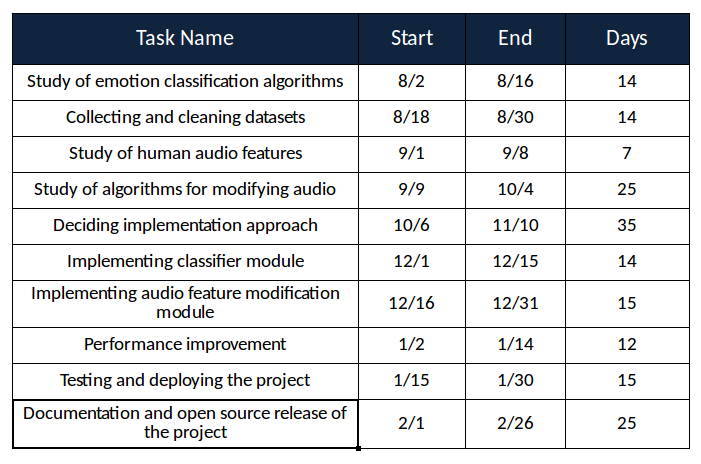
\includegraphics[width=470pt]{project_plan.png} \\



\chapter{Technical Keywords}
\section{Area of Project}
The project titled "Expressive English text-to-speech synthesis system" belongs to the domains of Machine Learning, Natural Language Processing and Digital Signal Processing. Since, we are trying to predict the emotions from text, a machine learning classifier is used for that purpose. Also, there are some cases wherein we have to check the sentence structure of prediction of emotions. This is where we use Natural Language Processing. Digital Signal Processing is required to modify neutral speech audio into affective audio.

\section{Technical Keywords}
% {\bfseries Technical Key Words:}      
% \begin{itemize}
%   \item[] 	Cloud Computing
% \item[]	Service Composition
% \item[]	Online Web services
% \end{itemize}
\begin{enumerate}
	\item[] F: Theory Of Computation 
	\begin{enumerate}
		\item[] F.2: ANALYSIS OF ALGORITHMS AND PROBLEM COMPLEXITY 
		\begin{enumerate}
			\item[] F.2.1: Numerical Algorithms and Problems (G.1, G.4, I.1) 
			\begin{enumerate}
				\item[]  B: Computations on matrices \\
						For TF-IDF representation, the feature vector of a particular sentence is represented as a sparse matrix using python scipy library. These matrices are then used for further calculations. In deep learning approach, the weights of a layer are internally represented using matrices. Various operations like convolution and element-wise addition are performed depending on the structure of the network.
			\end{enumerate}
		\end{enumerate}
		
	\end{enumerate}	 
	\item[] I: Computing Methodologies
	\begin{enumerate}
		\item[] I.2: ARTIFICIAL INTELLIGENCE
		\begin{enumerate}
			\item[] I.2.7: Natural Language Processing
			\begin{enumerate}
				\item[] A: Text analysis \\
						Text mining task of emotion detection is addressed in this project. It involves lexical analysis, part of speech tagging and term-weighting usng TF-IDF. For deep learning, word embeddings are used to map a word to a continuous vector space.\\
				\item[] B. Speech recognition and synthesis\\
						In this project we synthesize expressive speech from input text. Synthesized speech can be created by concatenating pieces of recorded speech that are stored in a database.
						Systems differ in the size of the stored speech units; a system that stores phones or diphones provides the largest output range, but may lack clarity.
						The two primary technologies generating synthetic speech waveforms are concatenative synthesis and formant synthesis.
						Concatenative synthesis is based on the concatenation (or stringing together) of segments of recorded speech.
						Formant synthesis does not use human speech samples at runtime. Instead, the synthesized speech output is created using additive synthesis and an acoustic model.
						Parameters such as fundamental frequency, voicing, and noise levels are varied over time to create a waveform of artificial speech.
						Many systems based on formant synthesis technology generate artificial, robotic-sounding speech that would never be mistaken for human speech. As our main motivation behind the
						project was to generate human-like speech we use concatenative synthesis method.\\
			\end{enumerate}
		\end{enumerate}
		\item[] I.5: PATTERN RECOGNITION
		\begin{enumerate}
			\item[] I.5.4: Applications
			\begin{enumerate}
				\item[] A. Signal Processing
						Signal Processing algorithms are used to perform operations on the neutral audio signal to synthesize expressive speech.
						Following are some of the functions performed:
						Speaking style and speaker identity adaptation supporting various voice conversion algorithms.
						Gaussian Mixture Model based voice conversion algorithms.
						Prosody transformation algorithms for voice conversion.
						Mean and standard deviation transformation of f0.
						Smoothing algorithms for voice conversion.
			\end{enumerate}
		\end{enumerate}
	\end{enumerate}		 
\end{enumerate} 

			
\chapter{Introduction}
\section{Project Idea}
To create a software program, which will take English language text as input and then will identify emotions of each and every sentence present in the text. It will try to speak the sentences such that the detected emotions are incorporated in the audio.


\section{Motivation behind the Project}  
The project group members are avid readers. We usually read novels and articles from various different sources. When we tried to use Adobe PDF reader's inbuilt 'read-out-aloud' feature for listening to the novel, we realized that it was highly monotonous and robotic in nature. This type of text-to-speech is unsuitable for listening to novels which are quite rich with different types of emotions. We then used some other text-to-speech engines like IvonaTTS, Jovie and KMouth (of Okular PDF reader). But the results were similar as that of Adobe PDF reader. Then we tried some other text-to-speech engines like MaryTTS and PSOLA. They have some ability to handle emotional audio synthesis, but they lack emotion detection facility. This inspired us to build a system which will first try to identify emotion associated with English text and then try to speak the sentences with emotions associated with it.

\section{Literature Survey}
\begin{enumerate}
	\item[\lbrack1\rbrack] Vanmassenhove, Eva, João P. Cabral, and Fasih Haider. "Prediction of emotions from text using sentiment analysis for expressive speech synthesis." 9th ISCA Speech Synthesis Workshop, Sunnyvale, USA, Septemper. 2016. \\\\
		 This paper presents a Text-to-speech engine which identifies emotions from text using a Machine Learning classifier. Then a voice is synthesized using Hidden Markov Modelling technique. The voice is modified using various emotions' characteristics classified using Self-Organizing Maps (SOM). The authors clain that it gives fairly good results in novels and fairy tales reading.
	\item[\lbrack2\rbrack] Perikos, Isidoros, and Ioannis Hatzilygeroudis. "Recognizing emotions in text using ensemble of classifiers." Engineering Applications of Artificial Intelligence 51 (2016): 191-201\\\\
	 This project extensively focusses on identifying emotions from English text. The authors have developed 2 classifiers, one Naive-Bayes and other is Max-entropy, for identification of emotions. Also, they have used Stanford Parser's Universal dependency for identifying sentence construction and then predicting the emotions. These three emotion prediction sub-systems then vote on the emotions they have retrieved and the emotion which gets maximum votes is selected as the overall emotion of the sentence.
	\item[\lbrack3\rbrack] Bowles Tristan, and Sandra Pauletto. "Emotions in the voice: humanising a robotic voice." Proceedings of the 7th Sound and Music Computing Conference, Barcelona, Spain. 2010\\\\
	The focus of this project is the manipulation of a robotic	voice signal for the purpose of adding emotional expression. In particular, its main aim was to design the emotion expressed by a robotic voice by manipulating specific acoustic parameters such as pitch, amplitude and speech rate. The three basic emotions considered were: anger, happiness and sadness.
		The technique of manipulating the accoustic parameters used in this paper will be helpful to implement the speech processing engine in our project. 
	\item[\lbrack4\rbrack] Pierre-Yves Oudeyer. “The production and recognition of emotions in speech: features and algorithms.” International Journal of Human-Computer Studies, 2003\\\\
	 This paper presents algorithms that allows a robot to express its emotions by modulating the
		intonation of its voice. It describes a technique which allows to
		continuously control both the age of a synthetic voice and the quantity of emotions that
		are expressed. Also, it presents the first large-scale data mining experiment about the
		automatic recognition of basic emotions in informal everyday short utterances. Its primary focused on
		the speaker-dependent problem.	
	\item[\lbrack5\rbrack] Sriram, S., \& Yuan, X. (2012, March). An enhanced approach for classifying emotions using customized decision tree algorithm. In Southeastcon, 2012 Proceedings of IEEE (pp. 1-6). IEEE.\\\\
	 In this paper a simple and memory optimized way for classifying emotions is discussed using customized decision tree.They have modified the already existing  Digg dataset and SemEval Affective Text-2007 by adding a new feature,emotion intensity.
	\item[\lbrack6\rbrack] Yong-Soo   seol,   Dong-Joo   Kim   and   Han-Woo   Kim,   "Emotion Recognition from Text using Knowledge-based ANN ", The 23'd International  Technical Conference  on Circuit/Systems, Computers and Communications. (lTS-CSCC-2008).\\\\
	 Yong-Soo Seol gives a hybrid method by incorporating knowledge-based method and machine learning method using artificial neural network for emotion detection.
	\item[\lbrack7\rbrack] Hsieh, Y. L., Liu, S. H., Chang, Y. C., \& Hsu, W. L. (2015, August). Neural Network-based Vector Representation of Documents for Reader-Emotion Categorization. In Information Reuse and Integration (IRI), 2015 IEEE International Conference on (pp. 569-573). IEEE.\\\\
	 In this paper emotion categorization using word embeddings is discussed on Chinese news corpus. Word embeddings can capture semantic context and can be used to infer similarity between words. This approach requires very little feature engineering and yields substantial success.
\end{enumerate}


\chapter{Problem Definition and scope}
\section{Problem Statement}
Develop a software program that reads a text file containing English sentences such that the emotions in the sentences are reflected in the audio.


\subsection{Goals and objectives}  
The goal of the project is to create a software system that will be able to identify emotions from english text and accordingly produce affective output.\\
There are two objectives associated with our project. First objective is to identify emotion associated with each and every sentence of the text. And the second objective is to modify neutral speech to incorporate emotion associated with the text.

 \subsection{Statement of scope}
 	The project aims at identifying 4 different emotions (happy, angry, sad and neutral) from the english text and producing speech that incorporates the emotions in the output. The input of the project is English text or English PDF file. The output of the project is speech signal with emotions of the text incorporated in it. Also, there are huge possibilities of construction a sentence with English language. Our scope is limited to identifying emotions of simple English sentences with arguably contains only one emotion. Only one negation is allowed in the sentence which can or cannot qualify the affective words in the sentence.

\section{Major Constraints}
 Large and accurate datasets for emotion classification using Machine Learning approaches are not available publicly because the researchers who create those datasets use university funding to crowdsource that job. We have used the datasets by requesting them for the same. So, dataset is extremely small by the standards required to train a highly accurate classifier.\\\\
 Machine Learning performs lot of computations on the input data while training the model. Due to unavailability of faster computing devices, the classifier model training takes enormous amount of time.\\\\
 Our system predicts only five different types of emotions namely, joy, sadness, surprise, anger and neutral due to the limitations posed by the dataset.\\\\
 As most of the novels, storybooks and scripts use text or Portable Document Format (PDF), our system supports only the aforementioned formats for input.\\\\
 The accent of the voice output of our system is US English. This is due to the dataset which we have used (CMU's Arctic voice dataset) to train the voice synthesis module.
 
\section{Methodologies of Problem solving and efficiency issues}
 Naive Bayes classification\\
 Naive Bayes requires a small number of training data to estimate the parameters necessary for classification.\\\\\\\\
LSTM classification\\ A LSTM network is universal in the sense that given enough network units it can compute anything a conventional computer can compute, provided it has the proper weight matrix, which may be viewed as its program.\\\\
Support vector machines\\ It can efficiently perform a non-linear classification by implicitly mapping their inputs into high-dimensional feature spaces.\\\\
HMM-based synthesis In this system , the frequency spectrum (vocal tract), fundamental frequency and duration of speech are modeled simultaneously by Hidden Markov Models.



\section{Outcomes}
 We define outcomes as the changes, benefits, learning or other effects that happen as a result of our work. The break-through achieved by our project is that it is the first end-to-end system which takes English text as input and produces affective output. Our work is multi-disciplinary in the sense that it extensively includes concepts and techniques from domains such as Machine Learning, Deep Learning, Natural Language Processing, Digital Signal Processing and High Performance Computing to name a few.

\section{Applications}
These days, the publisher not only publishes a printed version of the book but also releases an audio book. These audio books are generated by hiring voice actors in the recording studio where they read the entire book. Our project can work as an effective replacement for the process of audio book generation thereby saving both time and money of the publishers.\\\\
There are many PDF readers available which lack the emotional speech output producing capability for the novels and story books. These PDF readers can integrate our project by using an Application Programming Interface (API) and can effectively produce affective speech output.\\\\
Robots, these days, are now capable of speaking sentences in different languages. But their output is monotonous and devoid of any emotion. Our project's API can be used in the robots to eradicate this problem and thus, can help to make robots sound more human-like.

\section{Hardware Resources Required}
Our project requires following hardware resources to run smoothly and successfully 
\begin{table}[!htbp]
	\begin{center}
		\def\arraystretch{1.5}
		\begin{tabularx}{\textwidth}{| c | c | c | X |}
			\hline
			Sr. No. &	Parameter &	Min. Requirement & Justification \\
			\hline
			1 &	CPU Speed &	 1.0 GHz  & Fast processor required for fast proceesing\\
			\hline
			2 &	RAM  &	4 GB &  LSTM, Naive Bayes and NRC Lexicon model loading\\
			\hline
			3 & Audio output device & - & To listen to output audio\\
			\hline
		\end{tabularx}
		\caption { Hardware Requirements }
		\label{tab:hreq}
	\end{center}
	
\end{table}


\section{Software Resources Required}
Our project requires following software resources to run smoothly and successfully
\begin{table}[!htbp]
	\begin{center}
		\def\arraystretch{1.5}
		\begin{tabularx}{\textwidth}{| c | c | c | X |}
			\hline
			Sr. No. &	Parameter &	Suggested & Justification \\
			\hline
			1 &	Any Linux distribution &	 Ubuntu 16.04  & Easy dependency installation\\
			\hline
			2 &	Python  &	Python 2.7 & Stable and large community support against python 3.0\\
			\hline
			3 & MaryTTS & MaryTTS 5.2 & Advanced and stable signal processing functionalities\\
			\hline
			4 & NLTK & NLTK 3.2.2 & Provides English processing tools\\
			\hline
			5 & Scikit-learn & Scikit-learn 0.18.1 & Provides machine learning algorithms\\
			\hline
		\end{tabularx}
		\caption { Software Requirements }
		\label{tab:sreq}
	\end{center}
	
\end{table}




\chapter{Project Plan}

\section{Project Estimates}
\subsection{Reconciled Estimates}
\subsubsection{Cost Estimate}
Our project falls in organic class of software product.\\\\
For organic:\\
Effort = 2.4  * (KLOC)\textsuperscript{1.05}\\
\hspace*{12mm}=4.969271  PM\\\\\
Where,\\
KLOC is the estimated size of the software expressed in kilo\\ lines of code\\\\
Duration = 2.5 * (Effort)\textsuperscript{0.38}\\
\hspace*{18mm}= 4.5976  Months


\subsubsection{Time Estimates}
Learning about the tools, technologies and theory associated with our project which includes literature survey, Machine Learning, Deep Learning and Linguistic characteristics of Human speech took about 5 months.\\\\
Time required to implement the software system was about 2 months.



\subsection{Project Resources}
We have identified following three types of resources required for the successfull completion of our project within the stipulated time period.

	\subsubsection{Human Resources}
		\begin{enumerate}
			\item Internal Guide: Dr. Girish P. Potdar
			\item Group members:
				\begin{enumerate}[i]
					\item Pranjal Bhor
					\item Vaibhav Chaudhari
					\item Prathamesh Dharangutte
					\item Murtaza Raja
				\end{enumerate}
		\end{enumerate}
	
	\subsubsection{Hardware Resources}
		The following hardware resources were required during the incubation phase of our project
		\begin{table}[!htbp]
			\begin{center}
				\def\arraystretch{1.5}
				\begin{tabularx}{\textwidth}{| c | c | c | X |}
					\hline
					Sr. No. &	Parameter &	Required & Justification \\
					\hline
					1 &	CPU Speed &	 2.0 GHz  & Faster computation for training classifier\\
					\hline
					2 &	RAM  &	8 GB &  LSTM and Naive Bayes matrices temporary storage\\
					\hline
					3 & Nvidia GPU & GTX 860m & LSTM is neural network which requires GPU power to get trained\\
					\hline
					4 & Audio output device & - & To test the audio output\\
					\hline
				\end{tabularx}
				\caption { Hardware Requirements during incubation}
				\label{tab:incubhreq}
			\end{center}
			
		\end{table}
	\newpage
	\subsubsection{Software Resources}
		Following are the software resources required by our project while in its incubation phase
		\begin{table}[!htbp]
			\begin{center}
				\def\arraystretch{1.5}
				\begin{tabularx}{\textwidth}{| c | c | c | X |}
					\hline
					Sr. No. &	Parameter &	Suggested & Justification \\
					\hline
					1 &	Any Linux distribution &	 Ubuntu 16.04  & Easy dependency installation\\
					\hline
					2 &	Python  &	Python 2.7 & Stable and large community support against python 3.0\\
					\hline
					3 & MaryTTS & MaryTTS 5.2 & Advanced and stable signal processing functionalities\\
					\hline
					4 & NLTK & NLTK 3.2.2 & Provides English processing tools\\
					\hline
					5 & Scikit-learn & Scikit-learn 0.18.1 & Provides machine learning algorithms\\
					\hline
					6 & Nvidia CUDA & CUDA 8.0 & Provides drivers for running code on Nvidia GPU\\
					\hline
					7 & CudNN & CudNN v5.0 & Required to run Neural Network training algorithms on Nvidia GPU\\
					\hline
				\end{tabularx}
				\caption { Software Requirements during incubation }
				\label{tab:incubsreq}
			\end{center}
			
		\end{table}
	
\section{Risk Management w.r.t. NP Hard analysis}
\subsection{Risk Identification}
For risks identification, review of scope document, requirements specifications and schedule is done. Answers to questionnaire revealed some risks. Each risk is categorized as per the categories mentioned in Pressman. Please refer table \ref{tab:risk} for all the risks

\subsection{Risk Analysis}
The risks for the Project can be analyzed within the constraints of time and quality

\begin{table}[!htbp]
	\begin{center}
		%\def\arraystretch{1.5}
		\def\arraystretch{1.5}
		\begin{tabularx}{\textwidth}{| c | X | c | c | c | c |}
			\hline
			\multirow{2}{*}{ID} & \multirow{2}{*}{Risk Description}	& \multirow{2}{*}{Probability} & \multicolumn{3}{|c|}{Impact} \\ \cline{4-6}
			& & &	Schedule	& Quality	& Overall \\ \hline
			1	& Risk 1	& Medium	& Low	& Medium	& Medium \\ \hline
			2	& Risk 2	& Low	& Low	& Medium	& Medium \\
			\hline
			2	& Risk 3	& Medium	& Medium	& Medium	& Medium \\ \hline
		\end{tabularx}
	\end{center}
	\caption{Risk Table}
	\label{tab:risk}
\end{table}


\begin{table}[!htbp]
\begin{center}
%\def\arraystretch{1.5}
\def\arraystretch{1.5}
\begin{tabular}{| c | c | c |}
\hline
Probability & Value &	Description \\ \hline
High &	Probability of occurrence is &  $ > 75 \% $ \\ \hline
Medium &	Probability of occurrence is  & $26-75 \% $ \\ \hline
Low	& Probability of occurrence is & $ < 25 \% $ \\ \hline
\end{tabular}
\end{center}
\caption{Risk Probability definitions }
\label{tab:riskdef}
\end{table}

\begin{table}[!htbp]
\begin{center}
%\def\arraystretch{1.5}
\def\arraystretch{1.5}
\begin{tabularx}{\textwidth}{| c | c | X |}
\hline
Impact & Value	& Description \\ \hline
Very high &	$> 10 \%$ & Schedule impact or Unacceptable quality \\ \hline
High &	$5-10 \%$ & Schedule impact or Some parts of the project have low quality \\ \hline
Medium	& $ < 5 \% $ & Schedule impact or Barely noticeable degradation in quality Low	Impact on schedule or Quality can be incorporated \\ \hline
\end{tabularx}
\end{center}
\caption{Risk Impact definitions }
\label{tab:riskImpactDef}
\end{table}

\subsection{Overview of Risk Mitigation, Monitoring, Management}


Following are the details for each risk.
\begin{table}[!htbp]
	\begin{center}
		%\def\arraystretch{1.5}
		\def\arraystretch{1.5}
		\begin{tabularx}{\textwidth}{| l | X |}
			\hline 
			Risk ID	& 1 \\ \hline
			Risk Description	& If some of the words in the sentence are unknown to the classifier then the emotion of the sentence may not be identified correctly. \\ \hline
			Category	& Post-deployment \\ \hline
			Source	& Input text \\ \hline
			Probability	& Medium \\ \hline
			Impact	& Medium \\ \hline
			Response	& Mitigate \\ \hline
			Strategy	& Give only one emotion for the entire sentence \\ \hline
			Risk Status	&  Identified\\ \hline
		\end{tabularx}
	\end{center}
	%\caption{Risk Impact definitions \cite{bookPressman}}
	\label{tab:risk1}
\end{table}

\begin{table}[!htbp]
	\begin{center}
		%\def\arraystretch{1.5}
		\def\arraystretch{1.5}
		\begin{tabularx}{\textwidth}{| l | X |}
			\hline 
			Risk ID	& 2 \\ \hline
			Risk Description	& If all the words in the sentence are unknown to the classifier, then the sentence cannot be labelled. \\ \hline
			Category	& Post-deployment \\ \hline
			Source	& Input text \\ \hline
			Probability	& Low \\ \hline
			Impact	& Medium \\ \hline
			Response	& Mitigate \\ \hline
			Strategy	& Making classifier using larger dataset  \\ \hline
			Risk Status	& Identified \\ \hline
		\end{tabularx}
	\end{center}
	\label{tab:risk2}
\end{table}

\begin{table}[!htbp]
	\begin{center}
		%\def\arraystretch{1.5}
		\def\arraystretch{1.5}
		\begin{tabularx}{\textwidth}{| l | X |}
			\hline 
			Risk ID	& 3 \\ \hline
			Risk Description	& A sentence might contain more that one emotion which might make it difficult to process its audio. \\ \hline
			Category	& Development \\ \hline
			Source	& Classifier label \\ \hline
			Probability	& Medium \\ \hline
			Impact	& Medium \\ \hline
			Response	& Accept \\ \hline
			Strategy	& Processing audio using available technique  \\ \hline
			Risk Status	& Identified \\ \hline
		\end{tabularx}
	\end{center}
	\label{tab:risk3}
\end{table}

\section{Project Schedule}  
\subsection{Project task set} 
\begin{itemize}
	\item[]Task 1: Learning and understanding the basics of machine learning and digital signal processing techniques.
	\item[]Task 2: Generating a large dataset for emotion identification. 
	\item[]Task 3: Implementing and comparing various techniques available for speech processing and selecting the suitable one.
	\item[]Task 4: Creating a classifier that classifies the emotions in english text with reasonable accuracy.
	\item[]Task 5: Creating a speech signal processing module.
	\item[]Task 6: Combining speech signal processing module and classifier module to complete the system.
	\item[]Task 7: Testing and fixing of bugs in the system.
	\item[]Task 8: Documentation and open source release of the project.
\end{itemize}

\subsection{Task network}  
\vspace*{1\baselineskip}
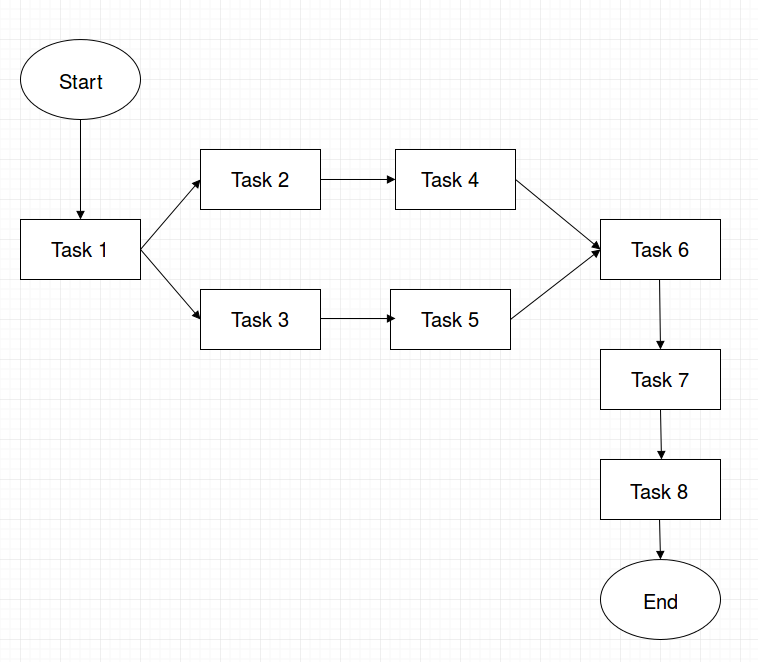
\includegraphics[width=400pt]{task_network.png}
\subsection{Timeline Chart}  
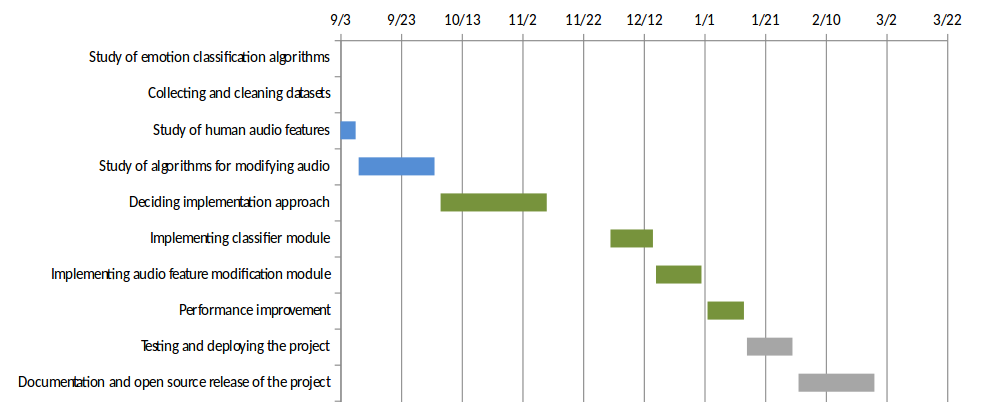
\includegraphics[height=300pt,width=480pt]{gantt_chart.png}

 
\section{Team Organization}  
\subsection{Team structure}
The team structure for the project is identified. Roles are defined.
\begin{itemize}
	\item[] Pranjal Bhor: Multi-threaded execution of the system and NLP emotion classifier developer.
	\item[] Vaibhav Chaudhari: Speech Synthesis System and signal processing developer.
	\item[] Prathamesh Dharangutte: Developer of Machine Learning based emotion classifier.
	\item[] Murtuza Raja: UI and NLP based emotion classifier developer.
\end{itemize}

\subsection{Management reporting and communication}
 E-mail\\
		It was used to communicate structural and design changes in the software to be developed. \\	\\	
 Whatsapp\\
		It was used to communicate in-short the work progress and status reporting\\\\
Verbal communication\\
		It was used for extensive discussion about the strategy, implementation and future to-do things about the project.

 
\chapter{Software requirement specification  }

\section{Introduction}
\subsection{Purpose and Scope of Document}
The purpose of this document is to present a detailed description of emotion labelling and speech signal processing mechanisms with a text-to-speech engine. It will explain the purpose and features of the system, the interfaces of the system, what the system will
do, and how the system will react to external stimuli. This document is intended for
both the users and the developers of the system.
This software system is designed to enhance the emotional aspect of the neutral text-to-speech engine. The system can be used by the PDF readers, audio books generating studios and video games companies to automate the reading of the english text. 

\subsection{Overview of responsibilities of Developer}
There are certain responsibilities which have to be taken care of by the developers of this project. First and foremost is to accurately define the scope and goals of the project. According to the scope, project design is made. Project plan of development is made. Each developer holds certain responsibility of specific module developement. The module development should contain novel approach to the problem encountered. Different types of testing are to be carried out on the final product made.
  
\section{Usage Scenario}
This section provides various usage scenarios for the system to be developed.  
\subsection{5.2.1 User profiles}  
\begin{itemize}
	\item[] \textbf{User}: User is the actor who uses the system. That is, user gives input to the system and gets the system's output.
	\item[] \textbf{Developer}: Developer is the actor who is responsible for designing, developing and maintaining the software system.
	\item[] \textbf{Researcher}: Researcher is responsible for formulating new features for the system, which are not currently available.
\end{itemize}

\subsection{Use-cases}
\begin{table}[!htbp]
	\begin{center}
		%\def\arraystretch{1.5}
		\def\arraystretch{1.5}
		\begin{tabularx}{\textwidth}{| c | c | X | c | X |}
			\hline
			Sr No.	& Use Case	& Description	& Actors	& Assumptions \\
			\hline
			1& English text input & The input file contains only the english text & User & The input is english text file \\
			\hline
			1& Non english text input & The input file contains non-english sentences & User & The input file contains english text \\
			\hline
		\end{tabularx}
	\end{center}
	\caption{Use Cases}
	\label{tab:usecase}
\end{table}


\subsection{Use Case View}
Use Case Diagram. Example is given below
\begin{center}
	\begin{figure}[!htbp]
		\hspace*{10pt}
		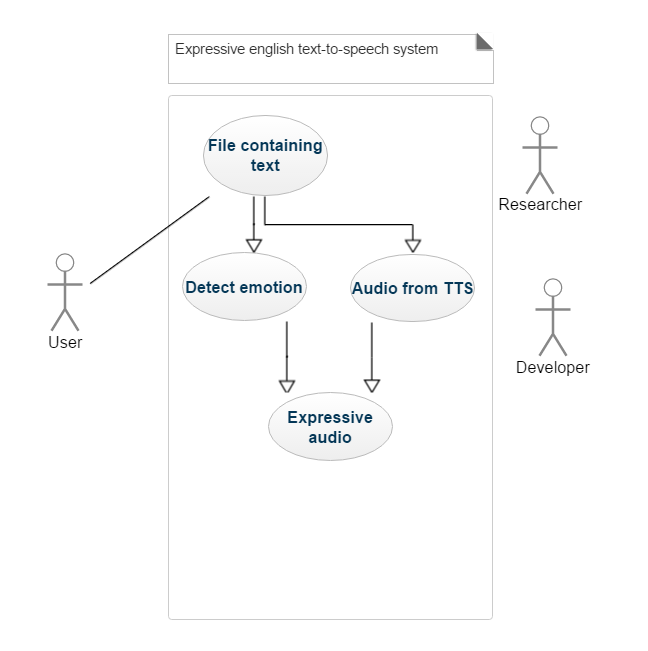
\includegraphics[width=340pt,height=230pt]{usecase.png}
		\caption{Use case diagram}
		\label{fig:usecase}
	\end{figure}
\end{center}  

\section{Data Model and Description}  
\subsection{Data Description}  
There are multiple types of data in the system. The machine learning classifier is a trained model which contains all the data on which it was trained along with its relationships with the output. The input data to the system consists of English text or PDF file. This data is to be loaded in memory in-order to work on it. Each and every sentence from the input file is to be classified into one of the 5 emotions. This also requires a data structure. The output of the system is audio data.  
\subsection{Data objects and Relationships}
The input to the system is English text or PDF file. The data that will be manipulated by the system is Neutral audio speech.
 
 
\section{Functional Model and Description}  

\subsection{Data Flow Diagram}
	\subsubsection{Level 0 Data Flow Diagram}
\begin{center}
	\begin{figure}[!htbp]
		\centering
		\includegraphics[scale=0.8]{dfdL0.png}
		\caption{Level 0 Data flow diagram}
		\label{fig:act-dig}
	\end{figure}
\end{center}

	\subsubsection{Level 1 Data Flow Diagram}
\begin{center}
	\begin{figure}[!htbp]
		\centering
		\includegraphics[scale=0.60]{dfdL1.png}
		\caption{Level 1 Data flow diagram}
		\label{fig:act-dig}
	\end{figure}
\end{center}

\subsubsection{Level 2 Data Flow Diagrams}
\begin{center}
	\begin{figure}[!htbp]
		\centering
		\includegraphics[scale=0.60]{dfdL20.png}
		\caption{Level 2 Data flow diagram - Emotion Classification}
		\label{fig:act-dig}
	\end{figure}
\end{center}

\begin{center}
	\begin{figure}[!htbp]
		\centering
		\includegraphics[scale=0.55]{dfdL21.png}
		\caption{Level 2 Data flow diagram - Speech Synthesis}
		\label{fig:act-dig}
	\end{figure}
\end{center}
 



 
\subsection{Activity Diagram:}
\begin{center}
	\begin{figure}[!htbp]
		\centering
		\fbox{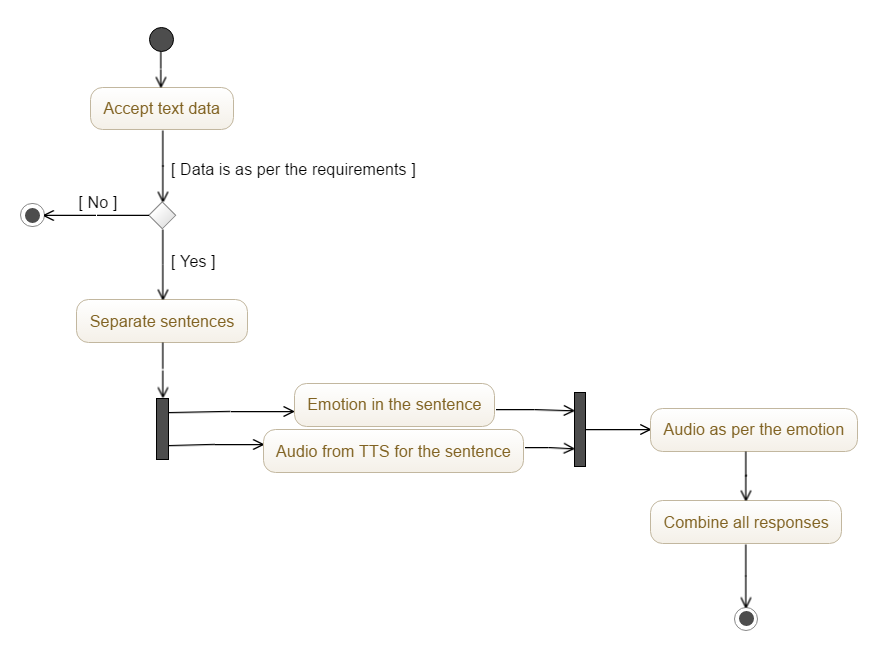
\includegraphics[height=330pt,width=400pt]{activity.png}}
		\caption{Activity diagram}
		\label{fig:act-dig}
	\end{figure}
\end{center} 

\subsection{Non Functional Requirements:}
Interface Requirements\\\\
The Graphical User Interface of the project should contain facility to select an English text or PDF file. It should also contain a mechanism to display the emotions of each and every sentence in the text file. There should be a media player type mechanism present in the system which the user can use to listen and seek the audio in-window. It can also contain facility to pause and stop the audio playing.\\\\
Performance Requirements\\\\
The system should be as fast as possible. The file loading and emotion detection phase should be extremely fast. Each sentence can be considered independently and so can processed through multi-threading. Similar goes for the audio genenration. Every sentence's audio can be generated independently of other sentences.\\\\
Software quality attributes\\\\
The software should be available all the time whenever user needs it. For a standalone software, it should be able to run whenever invoked. A web based application should have up-time of more than 99\%. The software should be reliable and should not give erratic or unwanted behaviour. It should be as modular as possible so that modifiability of the software can be improved. 

 \subsection{Design Constraints}	
There are no design constraints which will impact the subsystem. The software contains simple GUI as mentioned above and implementing that constraints the project developers in no significant way.

 \subsection{Software Interface Description}	 
 The software interface contains a mechanism through which an user will be able to load a file and can take an audio file of the input as the output. In the future, an Application Programming Interface (API) can be provided for the developers' use which will directly communicate with the comercially hosted servers.

\newpage
\subsection{State Diagram:}	
\begin{center}
	\begin{figure}[!htbp]
		\centering
		\fbox{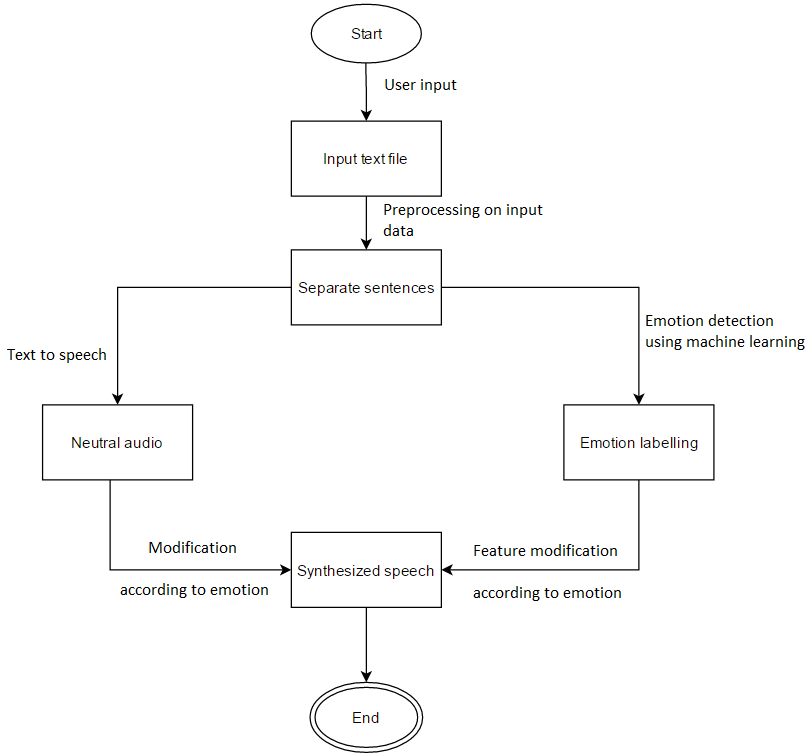
\includegraphics[width=400pt,height=290pt]{state.png}}
		\caption{State transition diagram}
		\label{fig:state-dig}
	\end{figure}
\end{center} 



\chapter{Detailed Design Document using Appendix A and B}
 \section{Introduction}  
This document specifies the design that is used to solve the problem of Product.  
\section{Architectural Design}  
	A description of the program architecture is presented.

 
  \begin{center}
	\begin{figure}[!htbp]
		\centering
		\fbox{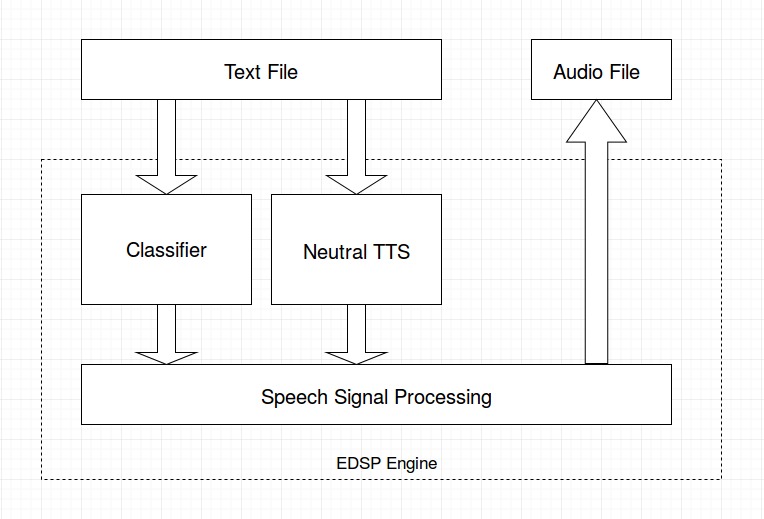
\includegraphics[width=400pt,height=300pt]{architechture.png}}
	  \caption{Architecture diagram}
	  \label{fig:arch-dig}
	\end{figure}
\end{center} 


\section{Data design (using Appendices A and B)}   
A description of all data structures including internal, global, and temporary data structures, database design (tables), file formats.
\subsection{Internal software data structure}
Multi-dimensional arrays\\\\
This data structure is used to store the machine learning classifier data. The classifier learns the data and maps it with the output. This mapping is stored in multi-dimensional arrays.\\\\
Dictionary\\\\
The input file contains many sentences. The emotions of these sentences are found out and they are stored in a dictionary where sentence is the key and its emotion is the value.
Tree\\\\
The system uses Stanford Parser to find out which phrases are qualified by specific words. The parser generates a parse tree out of the input English sentence.
\subsection{Global data structure}
There is no global data structure in the system. All the data sturctures are used internally by respective components.
\subsection{Database description}
Input data is stored in plain English text files or PDF files. Internally there is no use of database for handling of any types of tasks. The audio output is stored in .wav file format.

\newpage
\section{Component Design} 
\subsection{Class Diagram}
 \begin{center}
	\begin{figure}[!htbp]
		\centering
		\fbox{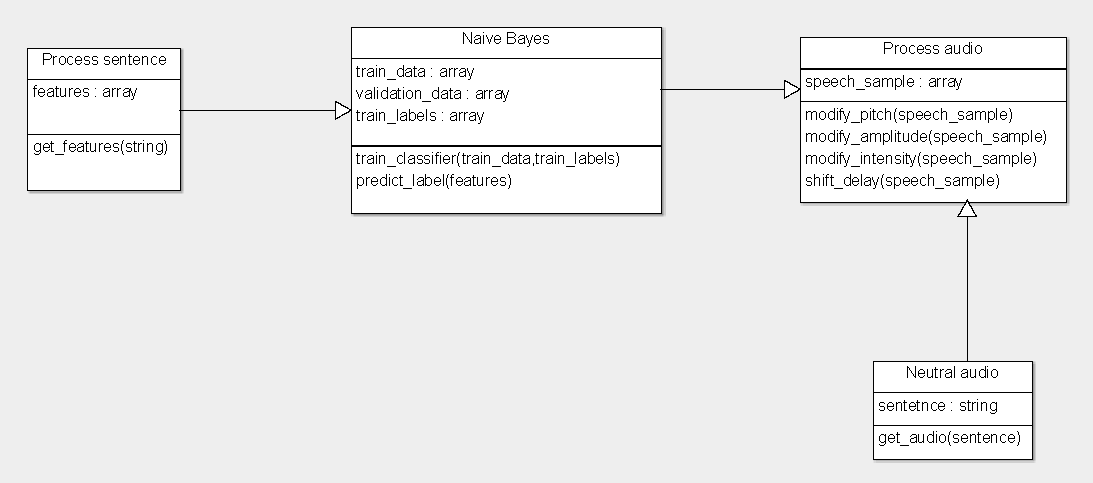
\includegraphics[width=450pt]{class_diagram.png}}
	  \caption{Class Diagram}
	  \label{fig:class-dig}
	\end{figure}
\end{center} 
 
\chapter{Project Implementation}
  \section{Introduction}
  Our system consists of a simple GUI wherein user has to load his text/PDF file containing English sentences. As soon as the file is loaded, each sentence from the file gets tagged with its most probable emotion. After clicking on speak button, affective audio for the sentences is generated and stored as a .wav file which is automatically played in the GUI. The user can control the audio file playing using a small media player provided.
  \section{Tools and Technologies Used}
   Python 2.7 Programming language\\\\\
   Python provides excellent libraries to automate most of the trivial work for system design. The members of the project group were already experienced in Python 2.7 and that is why we chose this as primary language for system implementation.\\\\
   MaryTTS signal processing engine\\\\
  	 MaryTTS is a research based Text-to-speech engine which supports many different languages including English. It has its own signal processing engine which modifies the neutral audio according to the input parameters given.
  	 This engine helps us to get emotional audio by modifying neutral audio.\\\\
  	 Festival\\\\
  	 It is a Hidden Markov Modelling (HMM) tool for building synthetic voice. As HMM is another form of machine learning, it requires training data in the form of voice audio and its text. As we want to have our own text-to-speech engine, we had to build our own voice which is why festival is used.\\\\
  	 NLTK and SCIKIT libraries\\\\
  	 NLTK contains many functions which carry out trivial tasks efficiently like stop words removal and tokenizing the words. It is also used to traverse on the parse tree generated by Stanford Parser. SCIKIT provides machine learning algorithms. We use the implementation of machine learning algorithms provided by SCIKIT python.
  	 
  \section{Methodologies/Algorithm Details}
  \subsection{Algorithms}
  \subsubsection{Overall System Algorithm}
	  \begin{algorithm}
	  	\caption{Overall system algorithm}
	  	\label{overall algorithm}
	  	\begin{algorithmic}[1]
	  		\Procedure{generate\_audio}{sentence}
	  		\State naive\_emotion $\leftarrow$ GET\_EMOTION\_FROM\_NAIVE(sentence)
	  		\State lstm\_emotion $\leftarrow$ GET\_EMOTION\_FROM\_LSTM(sentence)
	  		\State nlp\_emotion $\leftarrow$ GET\_EMOTION\_FROM\_NLP(sentence)
	  		\State final\_emotion $\leftarrow$ MOST\_VOTED\_EMOTION(naive emotion,lstm emotion,nlp emotion)
	  		\State neutral\_audio $\leftarrow$ HMM\_AUDIO\_SYNTHESIS(sentence)
	  		\State affective\ audio $\leftarrow$ SIGNALPROC(sentence,emotion)
	  		\State return save\ audio(affective audio)
	  		\EndProcedure
	  	\end{algorithmic}
	  	\begin{algorithmic}[1]
	  		\Procedure{sentence\_handler}{sentence}
	  		\State final\_audio = $\phi$
	  		\For {each sentence in text}
		  		\State temp\_audio $\leftarrow$ GENERATE\_AUDIO(sentence)
		  		\State final\_audio $\leftarrow$ final\_audio $\bigcup$ temp\_audio 
		  	\EndFor
	  		\EndProcedure
	  	\end{algorithmic}
	  \end{algorithm}
  
	\subsubsection{Naive Baye's Classification Algorithm}
		 \begin{algorithm}
			\caption{Naive Baye's Classification Algorithm}
			\label{NaiveBayes}
			\begin{algorithmic}[1]
				\Procedure{get\_emotion\_from\_naive}{sentence}
				\State classifier $\leftarrow$ load\_naive\_classifier()
				\State emotion $\leftarrow$ classifier.classify(sentence)
				\State return emotion
				\EndProcedure
			\end{algorithmic}
		\end{algorithm}
	
	\newpage
	\subsubsection{Get emotion from LSTM}
	\begin{algorithm}
		\caption{Get emotion from LSTM}
		\label{LSTM}
		\begin{algorithmic}[1]
			\Procedure{get\_emotion\_from\_lstm}{sentence}
			\State classifier $\leftarrow$ load\_lstm\_classifier()
			\State emotion $\leftarrow$ classifier.classify(sentence)
			\State return emotion
			\EndProcedure
		\end{algorithmic}
	\end{algorithm}

\subsubsection{HMM Audio Synthesis}
\begin{algorithm}
	\caption{HMM Audio Synthesis Algorithm}
	\label{HMMAudio}
	\begin{algorithmic}[1]
		\Procedure{HMM\_audio\_synthesis}{sentence}
		\State linguistic\_specification = get\_linguistic\_specification(sentence)
		\State final\_hmm\_sequence = $\phi$
		\ForAll{representation $\in$ linguistic\_specification}
		\State hmm\_sequence $\leftarrow$ generate\_hmm(representation)
		\State final\_hmm\_sequence $\leftarrow$ final\_hmm\_sequence $\cup$ hmm\_sequence
		\EndFor
		\State voice\_output $\leftarrow$ generate\_voice\_from\_hmm(final\_hmm)
		\State return voice
		\EndProcedure
	\end{algorithmic}
\end{algorithm}


	\subsubsection{Get emotion from NLP module}
	\begin{algorithm}
		\caption{Get emotion from NLP module}
		\label{NLP}
		\begin{algorithmic}[1]
			\Procedure{get\_emotion\_from\_nlp}{sentence}
			\State split sentence on spaces and store in word\_list
			\State word\_list $\leftarrow$ lemmatize(word\_list)
			\State word\_dictionary $\leftarrow$ $\phi$
			\For{each word in word\_list}
			\State word\_emotion $\leftarrow$ NRCclassifier(word)
			\State word\_dictionary\{word\} $\leftarrow$ word\_emotion
			\EndFor
			\algstore{myalg}
		\end{algorithmic}
	\end{algorithm}

	\begin{algorithm}
		\ContinuedFloat
		\caption{Get emotion from NLP module (continued)}
		\begin{algorithmic}
			\algrestore{myalg}
			
			\State emotion\_dictionary $\leftarrow$ \{'neutral':0,'joy':0,'sadness':0,'surprise':0,'anger':0\}
			\State dependency\_tree = StanfordParser(sentence)
			\State get\_index $\leftarrow$ 0
			\State Indices $\leftarrow$ $\phi$
			\For {each word in word\_dictionary}
			\State emotion\_dictionary\lbrack word\_dictionary[word]\rbrack += 20
			\State get\_index $\leftarrow$ find\_max\_qualified\_word(dependency\_tree)
			\For {$i$ = 0 and $i$<length(dependency\_tree)}
			\If {dependency\_tree[$i$].description is 'amod' or 'advmod'}
			\If {dependency\_tree[$i$].head = get\_index}
			\If {dependency\_tree[$i$].form in strong\_qual\_words}
			\State emotion\_dictionary\lbrack word\_dictionary[word]\rbrack += 100
			\ElsIf {dependency\_tree[$i$].form in avg\_qual\_words}
			\State emotion\_dictionary\lbrack word\_dictionary[word]\rbrack += 50
			\EndIf
			\EndIf
			\EndIf
			\EndFor
			\State Indices $\leftarrow$ Indices $\bigcup$ get\_index
			\EndFor
			\State answer\_emotion $\leftarrow$ get\_max\_valued\_emotion(emotion\_dictionary)
			\If {negation present in the sentence}
			\If {the negation word qualifies an index in Indices}
			\If {max\_emotion\_value $\>$ 20}
			\State answer\_emotion $\leftarrow$ 'neutral'
			\ElsIf {max\_emotion\_value == 20}
			\If {answer\_emotion == 'joy'}
			\State answer\_emotion $\leftarrow$ 'sadness'
			\ElsIf {answer\_emotion == 'sadness'}
			\State answer\_emotion $\leftarrow$ 'joy'
			\Else
			\State answer\_emotion $\leftarrow$ 'neutral'
			\EndIf
			\EndIf
			\EndIf
			\EndIf
			\State return emotion
			\EndProcedure
		\end{algorithmic}
	\end{algorithm}

  

  \section{Verification and Validation for Acceptance}
  Many different sentences denoting various emotions like joy, sadness, surprise, angry and neutral were given to the system. The system predicted the emotions and the people who tested the system agreed on the satisfactory level of the output. The corresponding audio generated was also approved by the users who tested the system. This provided verification as well as validation for the project and it got acceptance.
  
\chapter{Software Testing}
\section{Type of Testing Used}
Since our project focuses mainly on two important tasks – Classification of sentences based on emotions using machine learning (A) and conversion of monotonic speech into expressive speech (B), we have analyzed different testing strategies based on the aforementioned tasks.
\subsection{Unit testing}
This testing was very valuable for our project since we were able to independently test the emotion identification module and the speech synthesis module with good results. We essentially decoupled the two subsystems and tested them.
\subsubsection{Classification module}
This subsystem was tested by providing some sentences rich with five emotions - joy, sadness, anger,  surprise and neutral. With an accuracy of about 80\%, it produced the results accordingly. It labelled more sentences as neutral because the database was biased toward it.

\subsubsection{Speech synthesis module} 
For voice synthesis and digital signal processing unit, same sentences were given as input. The affective audio generated by the unit was perceived to contain the emotion tagged as reported by the test users. The sentences which depicted anger as the emotion, were spoken a bit fast by the system.

\subsection{Integration testing}
Having tested the individual subsystems, the emotion prediction and voice synthesis modules were then integrated. A sentence was passed to the input function of the system. The emotion classifier correctly identified the emotion tag of the sentence and then using this emotion tag, the affective audio was generated.
\subsubsection{Multithreading fix}
It was discovered during testing that a single MaryTTS engine does not handle simultaneous requests and is not thread safe. Therefore, we spawned multiple instances of the engine and then fired simultaneous requests to them.

\subsection{Validation testing}
Since the ideas presented through this project are still in research phase, a usable product is a feat that cannot be achieved provided the current technology in this field. Still, we tried to test this software, targeting the audio book publishers as our client.
\subsubsection{Emotional speech as output}
This software provides the affective audio for emotions - joy, sadness, anger, surprise and neutral for the input provided by the user.
\subsubsection{Input characteristics}
Since majority of text is either available as .txt or as .pdf, this software has the ability to process both of them.

\subsection{Performance and load testing}
We used load testing to test the system under various loads. The workstation on which testing was performed consisted of a 2.5 GHz quad-core machine with 8 GB of main memory running Ubuntu operating system.

\subsection{GUI testing}
We made a very simple GUI in the beginning but soon found out that it is not user friendly and does not have a native-look-and-feel. Then we made another GUI which solved the problems of the previous one and offered better functionality in terms of audio playing and emotion selection.
\subsubsection{Emotion selection}
A drop down menu was associated with each and every sentence that represented the emotion of the sentence. The user has the ability to change this according to his or her preference.
\subsubsection{Audio playback}
A media player like functionality was added to the GUI so that the user can play, pause, stop, seek and change the volume of the audio being played. 
\subsubsection{Scrollable interface}
If the number of sentences exceeded the minimum which can fit on the screen, the windows automatically provides scroll bars that can be used to navigate between the sentences.

\section{Test Cases and Results}
\subsection{Unit testing}
\subsubsection{Classifier module}   
\begin{table}[!htbp]
	\def\arraystretch{1.5}
	\begin{tabularx}{\textwidth}{|c|X|c|c|}
		\hline 
		No. & Input	& Expected Output & Actual Output \\ \hline
		1. & I am very delighted & joy & joy \\ \hline
		2. & My dog died & sadness & sadness \\ \hline
		3. & Oh my God, I got that! & surprise & surprise \\ \hline
		4. & I am very angry at that behaviour & anger & anger \\ \hline
		5. & Those were tough times for me & neutral & neutral \\ \hline
		6. & I am not happy & sadness & sadness \\ \hline
		7. & I am not very sad & neutral & neutral \\ \hline
	\end{tabularx}
	\caption{Test cases for classifier module}
	\label{tab:testcases}
\end{table}

\newpage
\subsubsection{Speech synthesis module}
\begin{table}[!htbp]
	\def\arraystretch{1.5}
	\begin{tabularx}{\textwidth}{|c|c|X|c|}
		\hline 
		No. & Input emotion	& Expected Output & Actual Output \\ \hline
		1. & joy& speaks in an overall pleasant way & as expected \\ \hline
		2. & sadness & the pitch drops and tempo decreases & as expected \\ \hline
		3. & surprise & the pitch increases, some words stressed & as expected \\ \hline
		4. & anger & speaks a bit fast & speaks very fast \\ \hline
		5. & neutral & speaks normally & as expected \\ \hline
	\end{tabularx}
	\caption{Test cases for speech synthesis module}
	\label{tab:testcases}
\end{table}

\subsection{Integration testing}
\begin{table}[!htbp]
	\def\arraystretch{1.5}
	\begin{tabularx}{\textwidth}{|c|X|X|c|}
		\hline 
		No. & Input	& Expected Output & Actual Output \\ \hline
		1. & affective sentence & emotional speech generated & as expected \\ \hline
		2. & neutral sentence & neutral speech generated & as expected \\ \hline
		3. & text file with various sentences & proper affective audio generated corresponding to emotions & as expected \\ \hline
		4. & pdf file with various sentences & proper affective audio generated corresponding to emotions & as expected \\ \hline
	\end{tabularx}
	\caption{Test cases for integration testing}
	\label{tab:testcases}
\end{table}

\newpage
\subsection{Validation testing}   
\begin{table}[!htbp]
	\def\arraystretch{1.5}
	\begin{tabularx}{\textwidth}{|c|X|c|X|}
		\hline 
		No. & Feature	& Implemented & Details \\ \hline
		1. & produces affective voice on emotional text input & yes & can process 5 emotions \\ \hline
		2. & handles text files & yes & can process .txt and .pdf \\ \hline
		3. & automatically tags sentences with emotions & yes & currently 80\% accurate \\ \hline
		4. & support for other languages & no & future scope, data set limitations \\ \hline
		5. & support for other accents & yes & training data to be provided \\ \hline
	\end{tabularx}
	\caption{Test cases for validation testing}
	\label{tab:testcases}
\end{table}

\subsection{Performance and load testing}   
\begin{table}[!htbp]
	\def\arraystretch{1.5}
	\begin{tabularx}{\textwidth}{|c|X|c|}
		\hline 
		No. & Input	& Time taken to execute \\ \hline
		1. & 5-10 sentences. & 2-3 seconds. \\ \hline
		2. & 1 page. & About 15 seconds. \\ \hline
		3. & 10-15 pages. & About 3 minutes. \\ \hline
		4. & A novel of about 300 pages. & About 1 hour 5 minutes. \\ \hline
		5. & 3-4 instances of our software running at the same time. & Sometimes system gets hung up. \\ \hline
	\end{tabularx}
	\caption{Test cases for load testing}
	\label{tab:testcases}
\end{table}

\newpage
\subsection{GUI testing}
\begin{table}[!htbp]
	\def\arraystretch{1.5}
	\begin{tabularx}{\textwidth}{|c|X|X|c|}
		\hline 
		No. & Case	& Expected Output & Actual Output \\ \hline
		1. & loading files & .txt and .pdf files loaded & as expected \\ \hline
		2. & changing emotion of a sentence & drop down updated & as expected \\ \hline
		3. & sentences overflow the viewport & proper scroll bars are added accrdingly & as expected \\ \hline
		4. & audio playing capability & play, pause, stop, seek, volume & as expected \\ \hline
		5. & performing computational intensive task & show progress to user & no progress shown \\ \hline
	\end{tabularx}
	\caption{Test cases for GUI testing}
	\label{tab:testcases}
\end{table}

\chapter{Results}
\section{Screenshots}
The welcome screen of our system looks as shown in Figure 10.1. It is a simple screen with some information about our project and the team members. It contains a only one button to load the English text file or PDF file.
 \begin{center}
 	\begin{figure}[!htbp]
 		\centering
 		\fbox{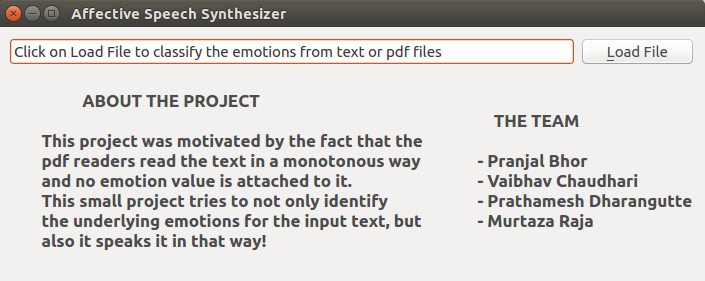
\includegraphics[width=450pt]{1.png}}
 		\caption{Intro screen}
 		\label{fig:intro-screen}
 	\end{figure}
 \end{center} 

When the file has been loaded in the interface, the emotions from each sentence are predicted and displayed in the GUI. The interface expands itself and adds new components to handle the sentences and their emotions. The size of the GUI increases because of this. Also, there is a selectable dropdown against each sentence which can be used by the user to change the emotion of the sentece if he/she is not satisfied by what is given by our classifier. This GUI is shown in Figure 10.2.
 \begin{center}
 	\begin{figure}[!htbp]
 		\centering
 		\fbox{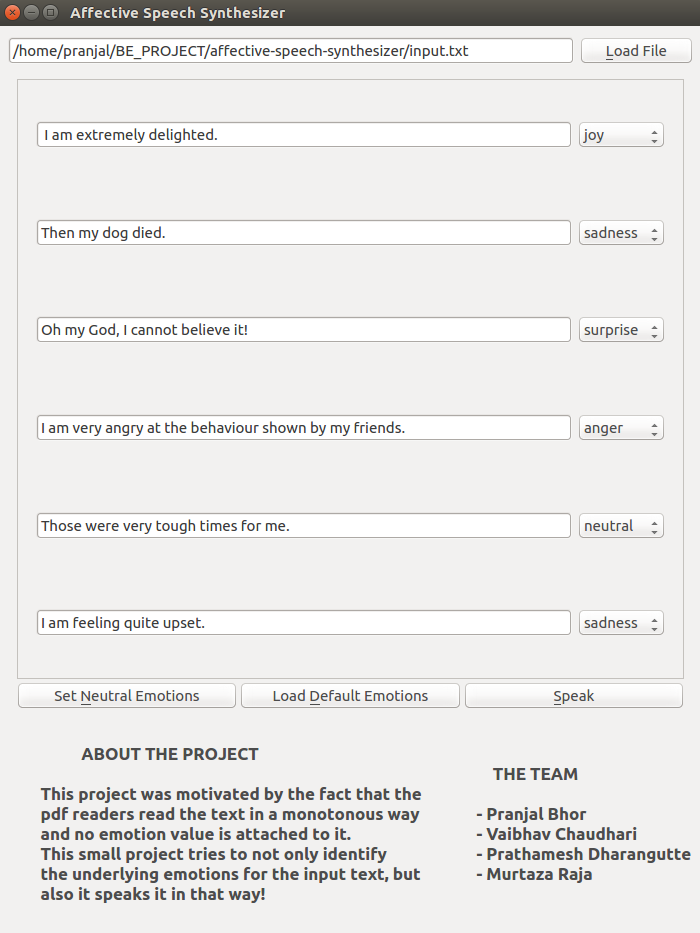
\includegraphics[width=450pt,height=500pt]{2.png}}
 		\caption{Emotion prediction screen}
 		\label{fig:Emotion prediction screen}
 	\end{figure}
 \end{center} 

\newpage 
After the emotions are predicted from the sentences, the user clicks on speak button. Then the affective audio of each and every sentence is generated and is automatically played by the software. A new component of media player is loaded for that purpose. The user can pause and stop the audio, can increase or decrease the volume and can even seek the slider to whatever position he wants.
  \begin{center}
  	\begin{figure}[!htbp]
  		
  		\fbox{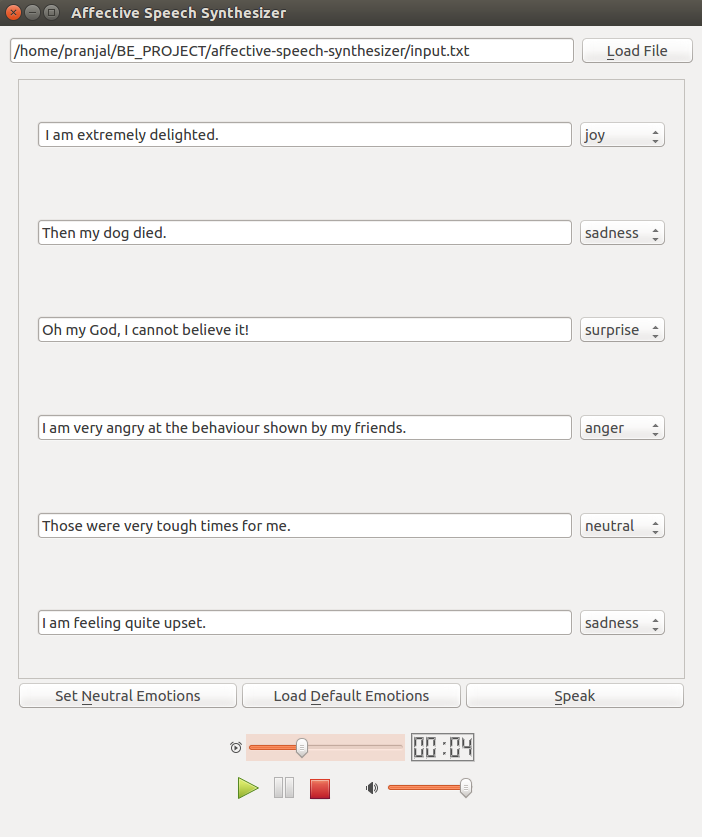
\includegraphics[width=450pt,height=430pt]{3.png}}
  		\caption{Affective audio playing screen}
  		\label{fig:Affective Audio playing screen}
  	\end{figure}
  \end{center} 

\chapter{Deployment and Maintenance}
     \section{Installation and un-installation}
     The program is a runnable python script. It does not require installation like a traditional software. But some dependencies have to be installed to run the software. The steps are as follows:
     \begin{enumerate}
     	\item Install project dependencies which includes: marytts-5.2, python 2.7, NLTK library, StanfordParser library, textract library, PyQT 4 and Phonon PyQT 4.
     	\item Download project source code
     	\item Execute 'run\_mary\_server.sh' script
     	\item Execute 'qtmain.py' script
     \end{enumerate}
     As there is no traditional installation associated with the system. The following steps are enough to remove the project from the system:
     \begin{enumerate}
     	\item Remove project dependencies which were installed in the installation steps.
     	\item Delete the project source code
     \end{enumerate}
 \chapter{Conclusion and future scope}
This project deals with the synthesis of expressive audio from the text. In this project we predict the emotion associated with a sentence and then generate audio corresponding to that audio and the sentence. The accuracy of the emotion prediction module is very important aspect in this process. Present techniques for emotion detection are not very accurate. So there is a tremendous scope for improvement in emotion detection. Currently, the system cannot effectively identify emotions of the sentences which contains words like 'rather' and 'but'. Some mechanism can be derived to handle such types of sentences. Building voices of characters according to their age, gender, background and other characteristics can be done using this project in the future.

% \bibliographystyle{plain}

\bibliographystyle{ieeetr}
\bibliography{biblo}

\begin{appendices}

\chapter{References}
\begin{itemize}
	\item[\lbrack1\rbrack] Vanmassenhove, Eva, João P. Cabral, and Fasih Haider. "Prediction of emotions from text using sentiment analysis for expressive speech synthesis." 9th ISCA Speech Synthesis Workshop, Sunnyvale, USA, Septemper. 2016.
	
	\item[\lbrack2\rbrack] M. Schröder and J. Trouvain (2003). The German Text-to-Speech Synthesis System MARY: A Tool for Research, Development and Teaching. International Journal of Speech Technology, 6, pp. 365-377.
	
	\item[\lbrack3\rbrack] Pierre-Yves, Oudeyer. "The production and recognition of emotions in speech: 	features and algorithms." International Journal of Human-Computer Studies 59.1 	(2003): 157-183.
	
	\item[\lbrack4\rbrack] Perikos, Isidoros, and Ioannis Hatzilygeroudis. "Recognizing emotions in text using ensemble of classifiers." Engineering Applications of Artificial Intelligence 51 (2016): 191-201.
	
	\item[\lbrack5\rbrack] Perikos, Isidoros, and Ioannis Hatzilygeroudis. "Recognizing emotion presence in natural language sentences." International Conference on Engineering Applications of Neural Networks. Springer Berlin Heidelberg, 2013.
	
	\item[\lbrack6\rbrack] Johnstone, Tom. The effect of emotion on voice production and speech acoustics. 	University of Western Australia, 2001.
	
	\item[\lbrack7\rbrack] Alm, Cecilia Ovesdotter, Dan Roth, and Richard Sproat. "Emotions from text: 	machine learning for text-based emotion prediction." Proceedings of the conference 	on human language technology and empirical methods in natural language 	processing. Association for Computational Linguistics, 2005.
	
	\item[\lbrack8\rbrack] Pang, Bo, and Lillian Lee. "Opinion mining and sentiment analysis." Foundations 	and trends in information retrieval 2.1-2 (2008): 1-135.
	
	\item[\lbrack9\rbrack] Christiane Fellbaum, Ed. 1998. WordNet: An Electronic Lexical Database. MIT 	Press, Cambridge, Mass. 
	
	\item[\lbrack10\rbrack] Chaffar, Soumaya, and Diana Inkpen. "Using a heterogeneous dataset for 	emotion analysis in text." Canadian Conference on Artificial Intelligence. Springer 	Berlin Heidelberg, 2011.
\end{itemize}

% \chapter{ALGORITHMIC DESIGN}
\chapter{Laboratory assignments on Project Analysis of Algorithmic Design}
\begin{center}
	\textbf{Assignment}
\end{center}
\begin{itemize}
\item[] To develop the problem under consideration and justify feasibilty using
concepts of knowledge canvas and IDEA Matrix.\\\\\\\\\\


\begin{table}[!htbp]
\begin{center}
  \begin{tabular}{| c | c | c | c |}
\hline
 I & D & E & A \\ 
\hline
Increase Accuracy & Drive Interaction & Educate Machine & Accelerate Processing\\
\hline
Improve Efficiency & Deliver Results & Evaluate Predictions & Associate Knowledge \\
 \hline
Ignore Risks & Decrease Errors & Eliminate Inaccuracy & Avoid Failure\\
\hline
\end{tabular}
 \caption { IDEA Matrix }
 \label{tab:imatrix}
\end{center}
\end{table}
\end{itemize}


\chapter{Project Planner}
\label{app:plan}
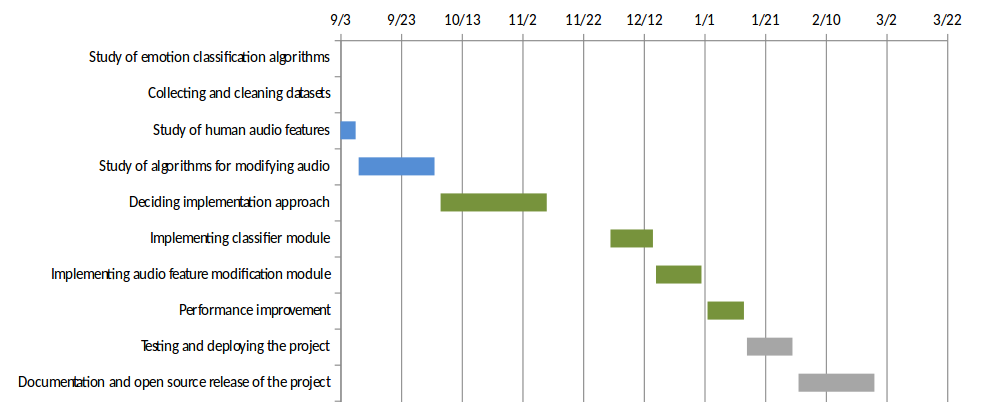
\includegraphics[height=300pt,width=480pt]{gantt_chart.png}



\chapter{Plagiarism Report}
Plagiarism report \\
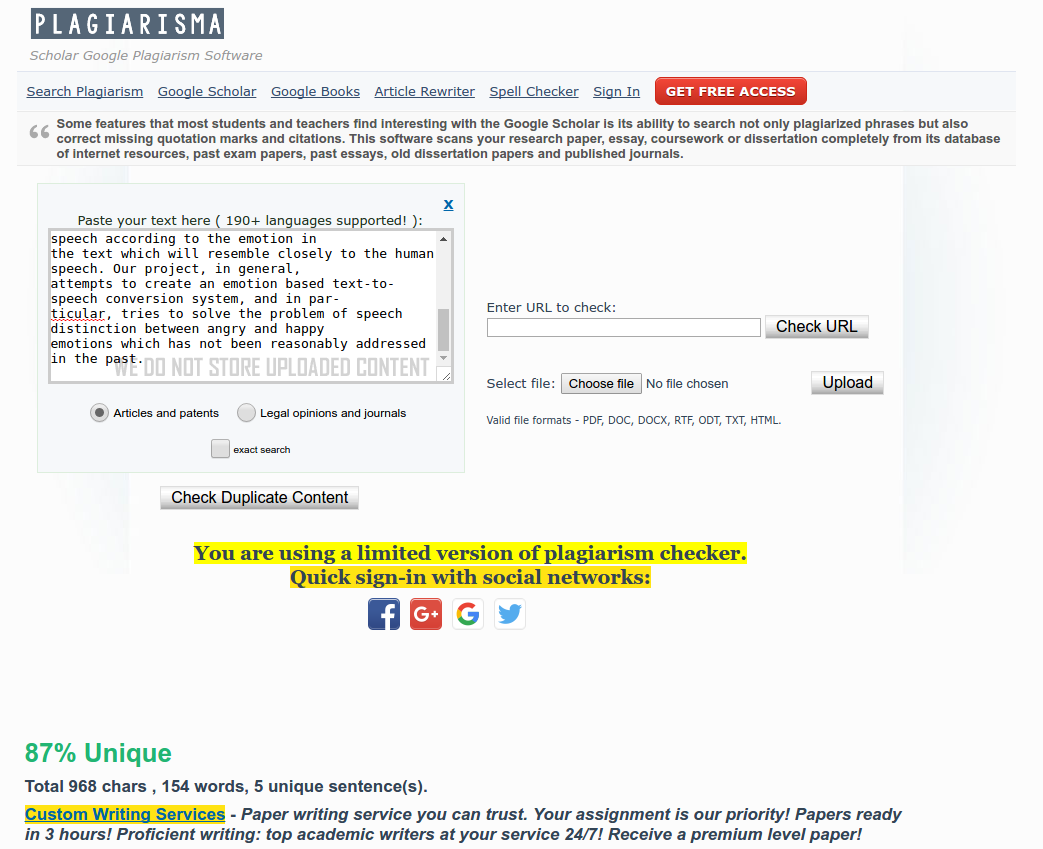
\includegraphics[width=400pt,height=450pt]{plagiarism.png}

\chapter{ Term-II Project Laboratory Assignments}
\begin{center}
	\textbf{Assignment 1}
\end{center}
Title: \\
Review of design and necessary corrective actions taking into consideration the feedback report of Term I assessment, and other competitions/conferences participated like IIT, Central Universities, University Conferences or equivalent centers of excellence etc. \\ \\
Earlier state of the project:\\
Simple sentences could be easily tagged with their emotions. But when some qualifying word comes, the emotion identification failed. It gave erratic results. \\\\
\begin{figure}[ht]
	\centering
	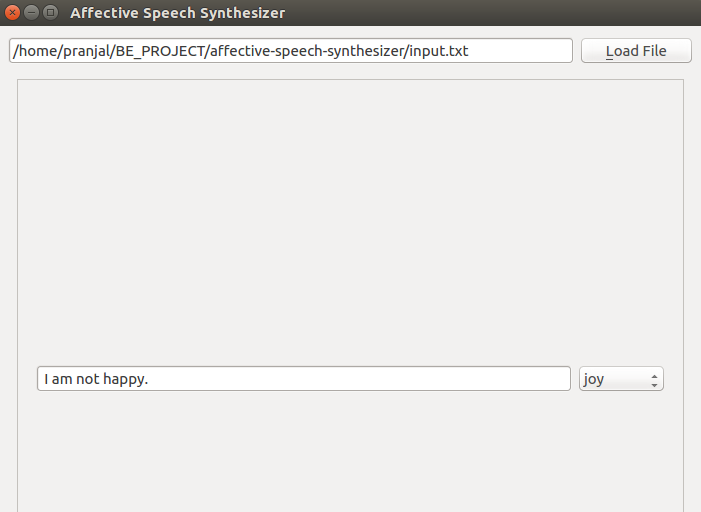
\includegraphics[width=400pt, height=340pt]{earlier.png}
	\caption{“I am not happy” wrongly classified as joy}
	\label{fig:“I am not happy” wrongly classified as joy}
\end{figure}

\newpage
After Corrective actions:\\
Sentences containing ‘not’ and qualifiers like ‘very’, ‘extremely’ are handled.\\\\
\begin{figure}[ht]
	\centering
	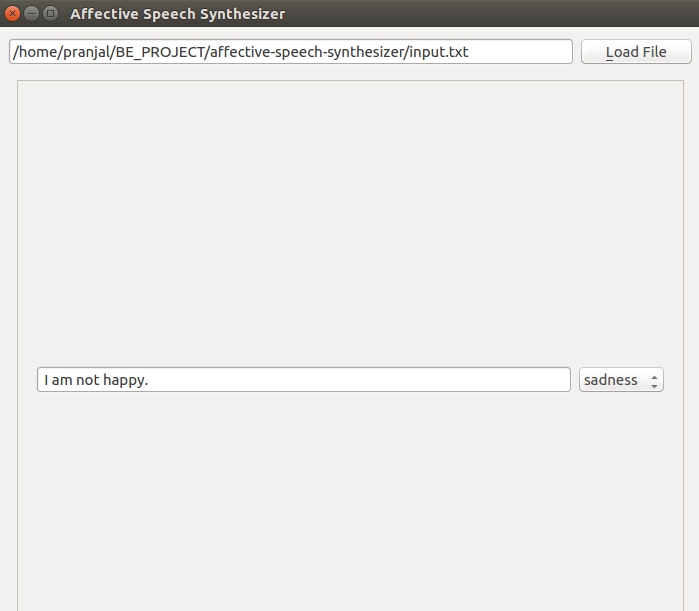
\includegraphics[width=400pt, height=340pt]{later.png}
	\caption{“I am not happy” correctly classified as sadness}
	\label{fig:“I am not happy” correctly classified as sadness}
\end{figure}

\newpage
\begin{center}
	\textbf{Assignment 2}
\end{center}
Title:\\
Project workstation selection, installations along with setup and installation report preparations.\\\\
Workstation Selection:\\
Platform – Linux platform is suitable because most of the dependencies of our software can be easily setup in it.\\
Number of cores in the machine – Multi-core system is preferable because our software exploits multithreading for faster execution.\\\\
Dependencies:
\begin{enumerate}
	\item[1.] marytts-5.2
	\item[2.] python 2.7
	\item[3.] NLTK library
	\item[4.] Stanford Parser library
	\item[5.] textract library
	\item[6.] PyQT 4
	\item[7.] Phonon PyQT 4
\end{enumerate}
Installation:
\begin{enumerate}
	\item[1.] Install project dependencies which includes: marytts-5.2, python 2.7,
	NLTK library, StanfordParser library, textract library, PyQT 4 and
	Phonon PyQT 4.
	\item[2.] Download project source code
	\item[3.] Execute 'run mary server.sh' script
	\item[4.] Execute 'qtmain.py' script
\end{enumerate}

\newpage
\begin{center}
	\textbf{Assignment 3}
\end{center}
Title:\\
 Programming of the project functions, interfaces and GUI (if any) as per 1 st Term term-work submission using corrective actions recommended in Term-I assessment of Term-work. \\ \\
 
\hspace*{0mm}Project GUI as per 1st Term term-work:\\ \\
\begin{figure}[ht]
	\centering
	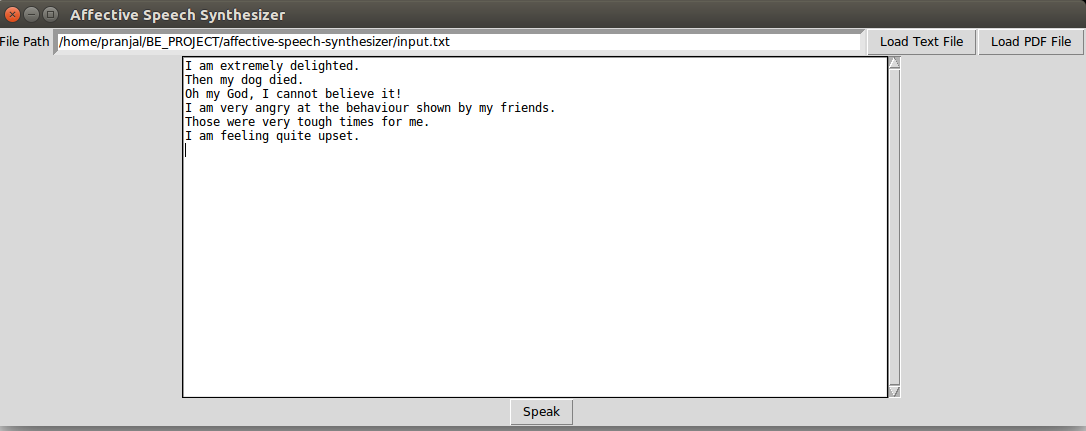
\includegraphics[width=400pt, height=340pt]{earlier_gui.png}
	\caption{Naive GUI made using python TKinter}
	\label{fig:Naive GUI made using python TKinter}
\end{figure}

\newpage
Project GUI after corrective actions suggested by project guide:\\\\
\begin{figure}[ht]
	\centering
	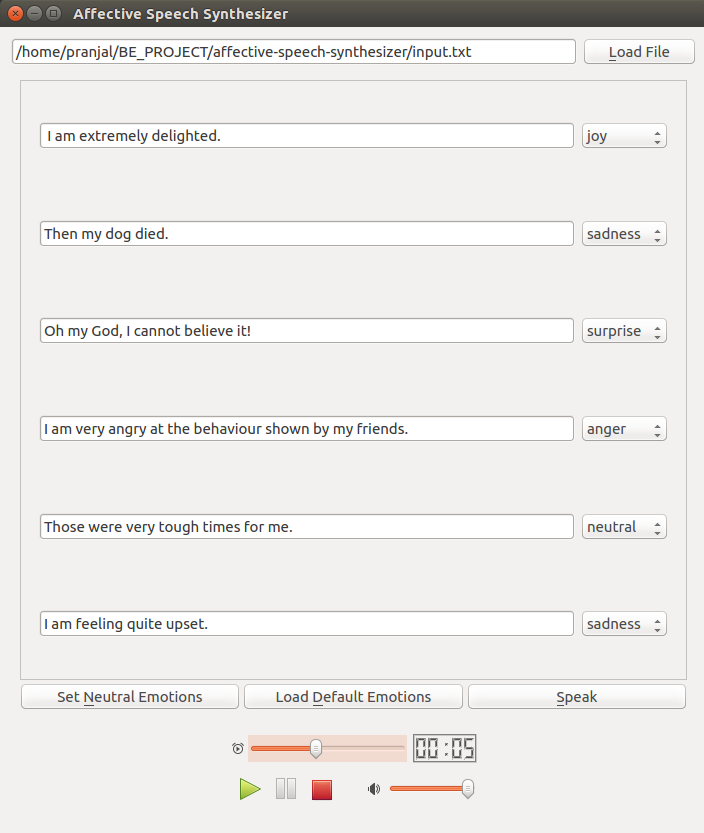
\includegraphics[width=400pt, height=400pt]{later_gui.png}
	\caption{Improved GUI with native look-and-feel}
	\label{Improved GUI with native look-and-feel}
\end{figure}

\newpage
\begin{center}
	\textbf{Assignment 4}
\end{center}
\section{Title}
Test tool selection and testing of various test cases for the project performed and generate various testing result charts, graphs etc. including reliability testing.
\section{Type of Testing Used}
Since our project focuses mainly on two important tasks – Classification of sentences based on emotions using machine learning (A) and conversion of monotonic speech into expressive speech (B), we have analyzed different testing strategies based on the aforementioned tasks.
\subsection{Unit testing}
This testing was very valuable for our project since we were able to independently test the emotion identification module and the speech synthesis module with good results. We essentially decoupled the two subsystems and tested them.
\subsubsection{Classification module}
This subsystem was tested by providing some sentences rich with five emotions - joy, sadness, anger,  surprise and neutral. With an accuracy of about 80\%, it produced the results accordingly. It labelled more sentences as neutral because the database was biased toward it.

\subsubsection{Speech synthesis module} 
For voice synthesis and digital signal processing unit, same sentences were given as input. The affective audio generated by the unit was perceived to contain the emotion tagged as reported by the test users. The sentences which depicted anger as the emotion, were spoken a bit fast by the system.

\subsection{Integration testing}
Having tested the individual subsystems, the emotion prediction and voice synthesis modules were then integrated. A sentence was passed to the input function of the system. The emotion classifier correctly identified the emotion tag of the sentence and then using this emotion tag, the affective audio was generated.
\subsubsection{Multithreading fix}
It was discovered during testing that a single MaryTTS engine does not handle simultaneous requests and is not thread safe. Therefore, we spawned multiple instances of the engine and then fired simultaneous requests to them.

\subsection{Validation testing}
Since the ideas presented through this project are still in research phase, a usable product is a feat that cannot be achieved provided the current technology in this field. Still, we tried to test this software, targeting the audio book publishers as our client.
\subsubsection{Emotional speech as output}
This software provides the affective audio for emotions - joy, sadness, anger, surprise and neutral for the input provided by the user.
\subsubsection{Input characteristics}
Since majority of text is either available as .txt or as .pdf, this software has the ability to process both of them.

\subsection{Performance and load testing}
We used load testing to test the system under various loads. The workstation on which testing was performed consisted of a 2.5 GHz quad-core machine with 8 GB of main memory running Ubuntu operating system.

\subsection{GUI testing}
We made a very simple GUI in the beginning but soon found out that it is not user friendly and does not have a native-look-and-feel. Then we made another GUI which solved the problems of the previous one and offered better functionality in terms of audio playing and emotion selection.
\subsubsection{Emotion selection}
A drop down menu was associated with each and every sentence that represented the emotion of the sentence. The user has the ability to change this according to his or her preference.
\subsubsection{Audio playback}
A media player like functionality was added to the GUI so that the user can play, pause, stop, seek and change the volume of the audio being played. 
\subsubsection{Scrollable interface}
If the number of sentences exceeded the minimum which can fit on the screen, the windows automatically provides scroll bars that can be used to navigate between the sentences.
\newpage
\section{Test Cases and Results}
\subsection{Unit testing}
\subsubsection{Classifier module}   
\begin{table}[!htbp]
	\def\arraystretch{1.5}
	\begin{tabularx}{\textwidth}{|c|X|c|c|}
		\hline 
		No. & Input	& Expected Output & Actual Output \\ \hline
		1. & I am very delighted & joy & joy \\ \hline
		2. & My dog died & sadness & sadness \\ \hline
		3. & Oh my God, I got that! & surprise & surprise \\ \hline
		4. & I am very angry at that behaviour & anger & anger \\ \hline
		5. & Those were tough times for me & neutral & neutral \\ \hline
		6. & I am not happy & sadness & sadness \\ \hline
		7. & I am not very sad & neutral & neutral \\ \hline
	\end{tabularx}
	\caption{Test cases for classifier module}
	\label{tab:testcases}
\end{table}

\newpage
\subsubsection{Speech synthesis module}
\begin{table}[!htbp]
	\def\arraystretch{1.5}
	\begin{tabularx}{\textwidth}{|c|c|X|c|}
		\hline 
		No. & Input emotion	& Expected Output & Actual Output \\ \hline
		1. & joy& speaks in an overall pleasant way & as expected \\ \hline
		2. & sadness & the pitch drops and tempo decreases & as expected \\ \hline
		3. & surprise & the pitch increases, some words stressed & as expected \\ \hline
		4. & anger & speaks a bit fast & speaks very fast \\ \hline
		5. & neutral & speaks normally & as expected \\ \hline
	\end{tabularx}
	\caption{Test cases for speech synthesis module}
	\label{tab:testcases}
\end{table}

\subsection{Integration testing}
\begin{table}[!htbp]
	\def\arraystretch{1.5}
	\begin{tabularx}{\textwidth}{|c|X|X|c|}
		\hline 
		No. & Input	& Expected Output & Actual Output \\ \hline
		1. & affective sentence & emotional speech generated & as expected \\ \hline
		2. & neutral sentence & neutral speech generated & as expected \\ \hline
		3. & text file with various sentences & proper affective audio generated corresponding to emotions & as expected \\ \hline
		4. & pdf file with various sentences & proper affective audio generated corresponding to emotions & as expected \\ \hline
	\end{tabularx}
	\caption{Test cases for integration testing}
	\label{tab:testcases}
\end{table}

\newpage
\subsection{Validation testing}   
\begin{table}[!htbp]
	\def\arraystretch{1.5}
	\begin{tabularx}{\textwidth}{|c|X|c|X|}
		\hline 
		No. & Feature	& Implemented & Details \\ \hline
		1. & produces affective voice on emotional text input & yes & can process 5 emotions \\ \hline
		2. & handles text files & yes & can process .txt and .pdf \\ \hline
		3. & automatically tags sentences with emotions & yes & currently 80\% accurate \\ \hline
		4. & support for other languages & no & future scope, data set limitations \\ \hline
		5. & support for other accents & yes & training data to be provided \\ \hline
	\end{tabularx}
	\caption{Test cases for validation testing}
	\label{tab:testcases}
\end{table}

\subsection{Performance and load testing}   
\begin{table}[!htbp]
	\def\arraystretch{1.5}
	\begin{tabularx}{\textwidth}{|c|X|c|}
		\hline 
		No. & Input	& Time taken to execute \\ \hline
		1. & 5-10 sentences. & 2-3 seconds. \\ \hline
		2. & 1 page. & About 15 seconds. \\ \hline
		3. & 10-15 pages. & About 3 minutes. \\ \hline
		4. & A novel of about 300 pages. & About 1 hour 5 minutes. \\ \hline
		5. & 3-4 instances of our software running at the same time. & Sometimes system gets hung up. \\ \hline
	\end{tabularx}
	\caption{Test cases for load testing}
	\label{tab:testcases}
\end{table}

\newpage
\subsection{GUI testing}
\begin{table}[!htbp]
	\def\arraystretch{1.5}
	\begin{tabularx}{\textwidth}{|c|X|X|c|}
		\hline 
		No. & Case	& Expected Output & Actual Output \\ \hline
		1. & loading files & .txt and .pdf files loaded & as expected \\ \hline
		2. & changing emotion of a sentence & drop down updated & as expected \\ \hline
		3. & sentences overflow the viewport & proper scroll bars are added accrdingly & as expected \\ \hline
		4. & audio playing capability & play, pause, stop, seek, volume & as expected \\ \hline
		5. & performing computational intensive task & show progress to user & no progress shown \\ \hline
	\end{tabularx}
	\caption{Test cases for GUI testing}
	\label{tab:testcases}
\end{table}

\begin{enumerate}
\item[] Emotion Classification testing\\
\begin{table}[!htbp]
	\begin{center}
		%\def\arraystretch{1.5}
		\def\arraystretch{1.5}
		\begin{tabularx}{\textwidth}{|X|c|c|}
			\hline 
			Input	& Expected Output & Actual Output \\ \hline
			I am very delighted & joy & joy \\ \hline
			My dog died & sadness & sadness \\ \hline
			Oh my God, I got that! & surprise & surprise \\ \hline
			I am very angry at that behaviour & anger & anger \\ \hline
			Those were tough times for me & neutral & neutral \\ \hline
			I am not happy & sadness & sadness \\ \hline
			I am not very sad & neutral & neutral \\ \hline
		\end{tabularx}
	\end{center}
	\label{tab:testcases}
\end{table}


\item[] Testing output audio quality:\\
For voice synthesis and digital signal processing unit, same sentences were given as input. The affective audio generated by the unit was perceived to contain the emotion tagged as reported by the test users.\\

\item[] Reliability Testing:\\
Load testing - We used load testing to test the system under various loads. The workstation o which testing was performed consisted of a 2.5 GHz quad-core machine with 8 GB of main memory and Ubuntu platform.\\\\

To this system varying loads were provided to check performance of the system.\\
\begin{table}[!htbp]
	\begin{center}
		%\def\arraystretch{1.5}
		\def\arraystretch{1.5}
		\begin{tabularx}{\textwidth}{|X|c|}
			\hline 
			Input	& Time taken to execute \\ \hline
			5-10 sentences. & 2-3 seconds. \\ \hline
			1 page. & About 15 seconds. \\ \hline
			10-15 pages. & About 3 minutes. \\ \hline
			A novel of about 300 pages. & About 1 hour 5 minutes. \\ \hline
			3-4 instances of our software running at the same time. & Sometimes system gets hung up. \\ \hline
		\end{tabularx}
	\end{center}
	\label{tab:testcases}
\end{table}
\end{enumerate}
\chapter{Information of Project Group Members}
\newpage

\begin{center}
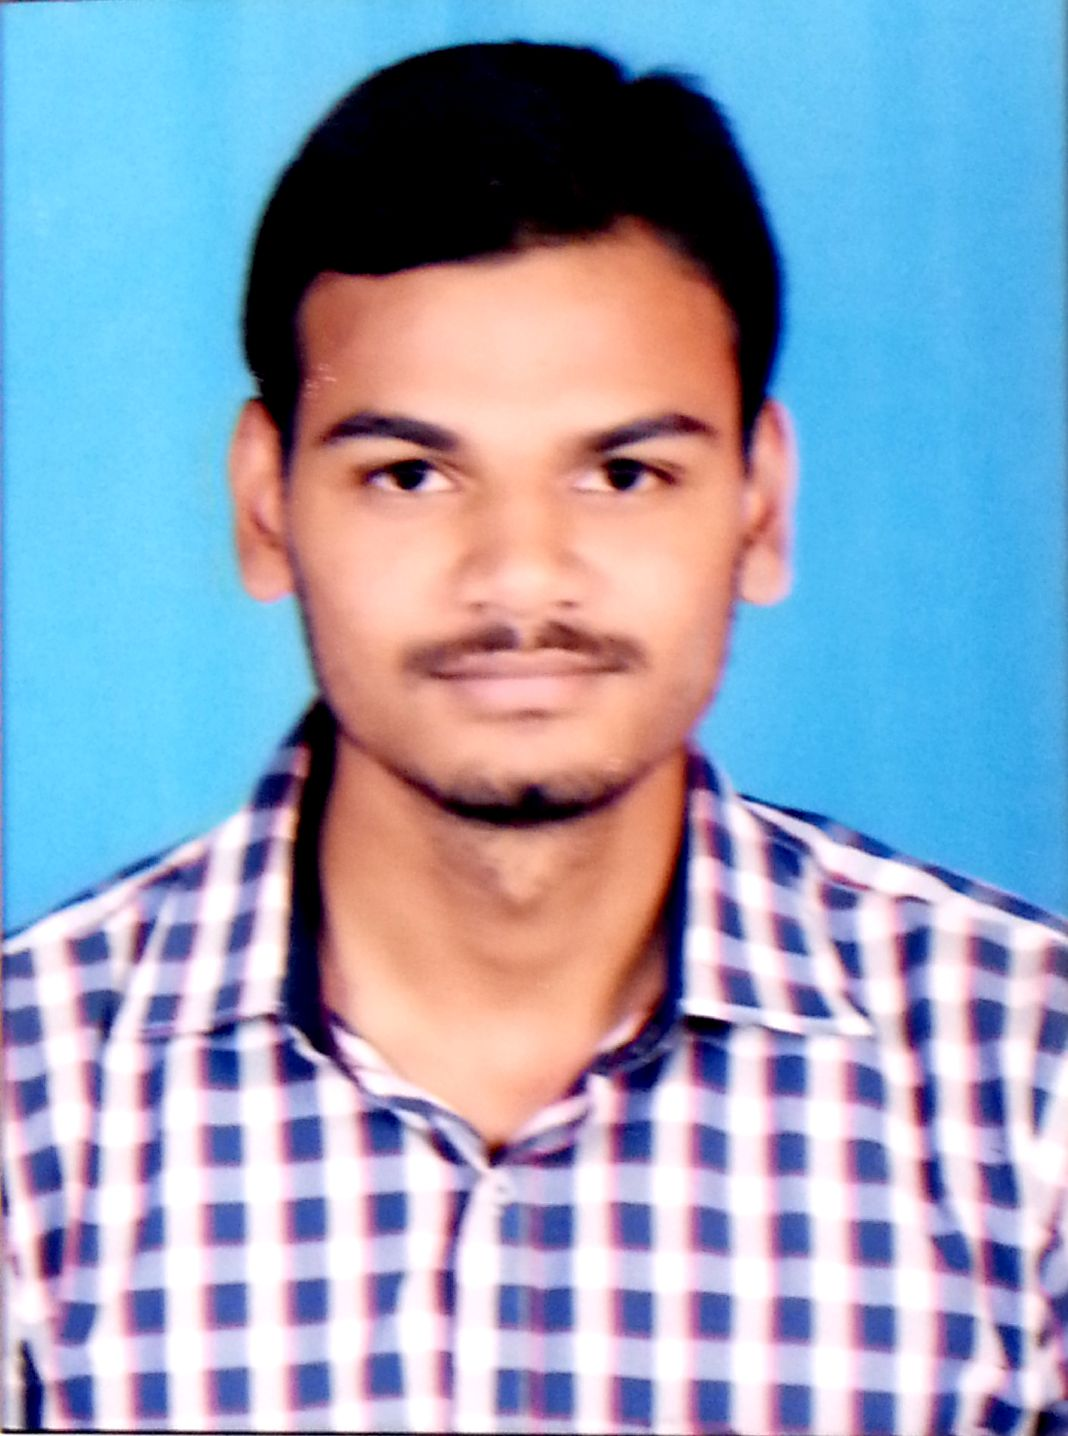
\includegraphics[width=60pt]{pranjal.jpg}
\end{center}
\begin{enumerate}
\item[] Name :  Pranjal Bhor\hspace{90 mm}
\item[] Date of Birth : Oct. 24th, 1994
\item[] Gender : Male
\item[] Permanent Address : Samartha housing society, shirsath mala, Savedi, Ahmednagar.
\item[] E-Mail : psmlbhor@gmail.com	
\item[] Mobile/Contact No. : +918698652268
\item[] Placement Details : Veritas Software
\end{enumerate}

\newpage

\begin{center}
	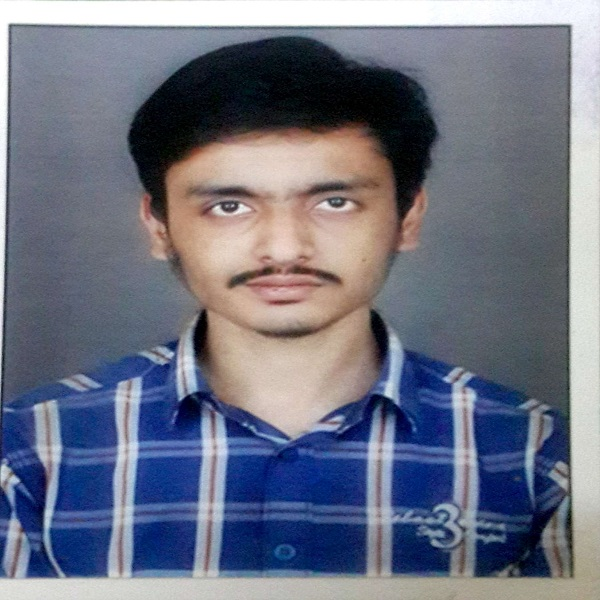
\includegraphics[width=60pt]{vaibhav.jpg}
\end{center}
\begin{enumerate}
	\item[] Name :  Vaibhav Chaudhari\hspace{90 mm}
	\item[] Date of Birth : April 24th, 1995
	\item[] Gender : Male
	\item[] Permanent Address : "Mruduprakash", Plot No. 19, Samartha Colony, near M.J. College,Jalgaon.
	\item[] E-Mail : vcvaibhav14@gmail.com	
	\item[] Mobile/Contact No. : +919403934320
	\item[] Placement Details : Tech Racers
\end{enumerate}

\newpage

\begin{center}
	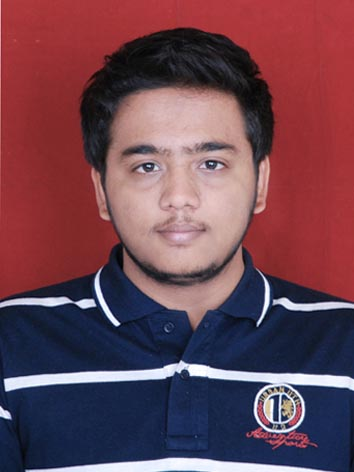
\includegraphics[width=60pt]{prathamesh.jpg}
\end{center}
\begin{enumerate}
	\item[] Name :  Prathamesh Dharangutte\hspace{90 mm}
	\item[] Date of Birth : May 18th, 1995
	\item[] Gender : Male
	\item[] Permanent Address : 13/357/1, Sona clinic, behind D-Mart, Datar mala, Kadapure Tal, Ichalkaranji. 
	\item[] E-Mail : pratham.d192@gmail.com	
	\item[] Mobile/Contact No. : +917588263102
	\item[] Placement Details : HSBC
\end{enumerate}

\newpage

\begin{center}
	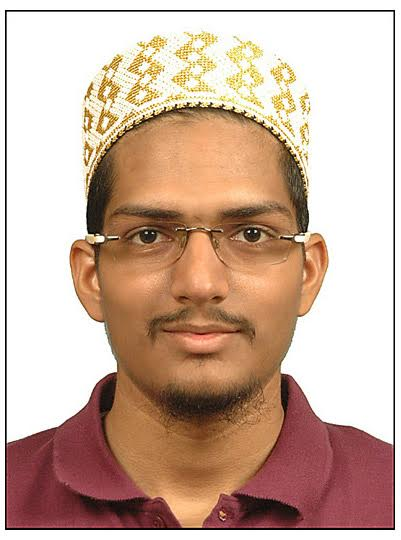
\includegraphics[width=60pt]{murtaza.jpg}
\end{center}
\begin{enumerate}
	\item[] Name :  Murtaza Raja\hspace{90 mm}
	\item[] Date of Birth : Jan. 15th, 1995
	\item[] Gender : Male
	\item[] Permanent Address : 102/A zainy bldg, shehabi colony, rustampura, nr. police chowky, Surat 395002
	\item[] E-Mail : murt.raja@gmail.com	
	\item[] Mobile/Contact No. : +918412806426
\end{enumerate}

\end{appendices}


\end{document}
